
\documentclass[oneside,a4paper]{book}

\usepackage{pdfpages}
%\pagestyle{headings}


%=============================================================================

\usepackage{amsthm}
\usepackage{xspace}
\usepackage{float}
\usepackage{ifthen}
\usepackage{amsbsy}
\usepackage{amssymb}
\usepackage{balance}
\usepackage{booktabs}
\usepackage{graphicx}
\usepackage{rotating}
\usepackage{multirow}
\usepackage{needspace}
\usepackage{microtype}
\usepackage{bold-extra}
\usepackage{geometry}
\usepackage{varioref}
\usepackage{xcolor}
\usepackage{textcomp}
\usepackage{listings}
\usepackage[normalem]{ulem} %emphasize still italic
\usepackage{ucs}
\usepackage{pdflscape}
\usepackage{graphicx}
\usepackage{longtable}
\usepackage{float}
\usepackage{multirow}
\usepackage{tikz}
\usepackage{array}
\usetikzlibrary{shapes.callouts, positioning, shapes, arrows.meta, fit}


% \usepackage[utf8]{inputenc}
% \usepackage[htt]{hyphenat}
\usepackage{times}
\usepackage{url}
\usepackage{alltt}
\usepackage{amsmath}
\usepackage{xfrac}
\usepackage{subfigure}
\usepackage{appendix}
\usepackage{stmaryrd}   % for the \shortuparrow
\usepackage[utopia]{quotchap}

\usepackage{setspace}
\usepackage[numbers, sort&compress]{natbib}
\usepackage{mdwlist}        % support for better spaced lists
% allows for temporary adjustment of side margins
\usepackage{chngpage}
\usepackage[normalem]{ulem} 
\usepackage{tikz}
\usetikzlibrary{shapes, arrows.meta, positioning}

\tikzset{
  block/.style={rectangle, draw=black, fill=yellow!50, rounded corners, minimum height=1.2em, text centered, text width=3cm},
  module/.style={circle, draw=black, fill=blue!30, minimum size=2cm, text centered, align=center}, 
  orchestrator/.style={circle, draw=black, fill=black, text=white, minimum size=2.5cm, text centered},
  arrow/.style={-Stealth, thick}
}

% constants

\newcounter{qcounter}

% commands
\newcommand{\n}{$\cdot$}
\newcommand{\y}{\checkmark}
\newcommand{\subscript}[1]{$_{\textrm{\footnotesize{#1}}}$}
\newcommand{\superscript}[1]{$^{\textrm{\footnotesize{#1}}}$}
\newcommand{\vertical}[1]{\raisebox{-4em}{\begin{sideways}{#1}\end{sideways}}}

\newboolean{showedits}
\setboolean{showedits}{true} % toggle to show or hide edits
\ifthenelse{\boolean{showedits}}
{
       \newcommand{\ugh}[1]{\textcolor{red}{\uwave{#1}}} % please rephrase
       \newcommand{\ins}[1]{\textcolor{blue}{\uline{#1}}} % please insert
       \newcommand{\del}[1]{\textcolor{red}{\sout{#1}}} % please delete
       \newcommand{\chg}[2]{\textcolor{red}{\sout{#1}}{\ra}\textcolor{blue}{\uline{#2}}} % please change
}{
       \newcommand{\ugh}[1]{#1} % please rephrase
       \newcommand{\ins}[1]{#1} % please insert
       \newcommand{\del}[1]{} % please delete
       \newcommand{\chg}[2]{#2}
}


% ============================================================================
% Put edit comments in a really ugly standout display

\usepackage{xcolor}
\usepackage[normalem]{ulem}
\newcommand{\ra}{$\rightarrow$}


% comments \nb{label}{color}{text}
\newboolean{showcomments}
\setboolean{showcomments}{true}
\ifthenelse{\boolean{showcomments}}
    {\newcommand{\nb}[3]{
        {\colorbox{#2}{\bfseries\sffamily\scriptsize\textcolor{white}{#1}}}
        {\textcolor{#2}{\sf\small$\blacktriangleright$\textit{#3}$\blacktriangleleft$}}}
     \newcommand{\version}{\emph{\scriptsize$-$Id$-$}}
%	 \newcommand{\ugh}[1]{\textcolor{red}{\uwave{#1}}} % please rephrase
%	 \newcommand{\ins}[1]{\textcolor{blue}{\uline{#1}}} % please insert
%	 \newcommand{\del}[1]{\textcolor{red}{\sout{#1}}} % please delete
%	 \newcommand{\chg}[2]{\textcolor{red}{\sout{#1}}{\ra}\textcolor{blue}{\uline{#2}}} % please change
	 \newcommand{\chk}[1]{\textcolor{ForestGreen}{#1}} % changed, please check
	}
    {\newcommand{\nb}[3]{}
     \newcommand{\version}{}
	\newcommand{\chk}[1]{} % changed, please check
	}

% ============================================================================
% Make quotes be italic
\renewenvironment{quote}
    {\list{}{\rightmargin\leftmargin}%
     \item\relax\begin{it}}
    {\end{it}\endlist}

\newcommand{\ttimes}{\ensuremath{\times}}

%=============================================================================

\newcommand{\needlines}[1]{\Needspace{#1\baselineskip}}

% source code
\usepackage{xcolor}
\usepackage{textcomp}
\usepackage{listings}
\definecolor{source}{gray}{0.9}
\lstset{
	language={},
	% characters
	tabsize=3,
	upquote=true,
	escapechar={!},
	keepspaces=true,
	breaklines=false,
	alsoletter={:},
	breakautoindent=true,
	columns=fullflexible,
	showstringspaces=false,
	basicstyle=\footnotesize\ttfamily,
	% background
	frame=single,
    framerule=0pt,
	backgroundcolor=\color{source},
	% numbering
	numbersep=5pt,
	numberstyle=\tiny,
	numberfirstline=true,
	% captioning
	captionpos=b,
	numberbychapter=false,
	% formatting (html)
	moredelim=[is][\textbf]{<b>}{</b>},
	moredelim=[is][\textit]{<i>}{</i>},
	moredelim=[is][\uline]{<u>}{</u>}}
\newcommand{\ct}{\lstinline[backgroundcolor=\color{white},basicstyle=\footnotesize\ttfamily]}
\newcommand{\lct}[1]{{\small\tt #1}}


%----------------------------------------------------------------------------
% references
\newcommand{\tabref}[1]{\hyperref[{tab:#1}]{Table~\ref*{tab:#1}}}
\newcommand{\figref}[1]{\hyperref[{fig:#1}]{Figure~\ref*{fig:#1}}}
\newcommand{\secref}[1]{\hyperref[{sec:#1}]{Section~\ref*{sec:#1}}}
\newcommand{\lstref}[1]{\hyperref[{lst:#1}]{Listing~\ref*{lst:#1}}}
\newcommand{\charef}[1]{\hyperref[{cha:#1}]{Chapter~\ref*{cha:#1}}}
%----------------------------------------------------------------------------

% abbreviations
\tracingcolors 4
\setcounter{tocdepth}{3}
\setcounter{secnumdepth}{3}
\newcommand{\ie}{\emph{i.e.,}\xspace}
\newcommand{\eg}{\emph{e.g.,}\xspace}
\newcommand{\etc}{\emph{etc.}\xspace}
\newcommand{\etal}{\emph{et al.}\xspace}


\newcommand{\newevenside}{
	\ifthenelse{\isodd{\thepage}}{\newpage}{
	\newpage
        \phantom{placeholder} % doesn't appear on page
	\thispagestyle{empty} % if want no header/footer
	\newpage
	}
}

\def\stretchfactor{1}
\newcommand{\mychapter}[1]{\setstretch{1}
    \chapter{#1}\setstretch{\stretchfactor}}

%----------------------------------------------------------------------------
\newcommand{\lessSpace}{\vspace{-1em}}
\DeclareGraphicsExtensions{.pdf,.png}
\graphicspath{{images/}}
\newcommand{\fig}[4]{
	\begin{figure}[#1]
		\centering
		\includegraphics[width=#2\textwidth]{#3}
		\lessSpace
		\caption{\label{fig:#3}#4}
	\end{figure}}

% ===========================================================================


\newcommand{\thesistitle}{Evaluating the Effects of Experiencing a Mixed Reality Simulation of Symptoms of Schizophrenia on Empathy in Medical Students}
\newcommand{\thesisauthor}{Ann Kiener}
\newcommand{\thesisleiter}{Prof. Elena Mugellini}
\newcommand{\thesisasst}{Prof. Denis Lalanne}
\newcommand{\thesissubtitle}{Thesis subtitle}
\newcommand{\thesisdate}{\today}



% ===========================================================================

\usepackage[ colorlinks=true, urlcolor=black, linkcolor=black,
			citecolor=black, bookmarksnumbered=true, bookmarks=true,
			plainpages=false,
			pdftitle={\thesistitle}, pdfauthor={\thesisauthor},
			pdfsubject={\thesissubtitle}, pdfpagelabels]{hyperref}

\newcommand{\hrref}[2]{\hyperref}
% ===========================================================================
% ===========================================================================


% D O C U M E N T
% % % % % % % % % % % % % % % % % % % % % % % % % % % % % % % % % %
\begin{document}

% T I T L E
% % % % % % % % % % % % % % % % % % % % % % % % % % % % % % % % % %
\begin{titlepage}  
  \begin{center}  
  
  \begin{figure}[t]  
  \vspace*{-2cm}        % to move header logo at the top 
  \center{
\includegraphics[scale=0.2]{logos/MSc_quer.png}}
  \vspace{0.4in}     
  \end{figure}

    \thispagestyle{empty}
    
    {\bfseries\Huge \thesistitle \par}
    %\Large \vspace{0.1in} \thesissubtitle \par}

    \vspace{0.3in} 
    \LARGE{\textbf{Master Thesis} \\}
    \vspace{0.4in}

    {\Large \thesisauthor}
    
    \vspace{0.3in}
    {\Large University of Bern \par}
%    {\Large Philosophisch-naturwissenschaftlichen Fakult\"{a}t \\
%            der Universit\"{a}t Bern \par}
    \vspace{0.3in}
    {\Large \emph{supervised by} \par}
    {\Large \thesisleiter \par}
    {\Large \thesisasst \par}
    \vfill
    {\Large \thesisdate \par}
    
  

  \vspace{0.9in}
 
  % === Logos ==============================================     
  \begin{figure}[htp]
    \centering
    
\includegraphics[scale=0.30]{logos/UNI_Bern.png}\hfill
    
\includegraphics[scale=0.30]{logos/UNI_Neuenburg.png}\hfill
    
\includegraphics[scale=0.80]{logos/UNI_Fribourg.png}
  \end{figure}
  % === // Logos ===========================================    


  \end{center}

\end{titlepage}


% A B S T R A C T
% % % % % % % % % % % % % % % % % % % % % % % % % % % % % % % % % %
\chapter*{\centering Abstract}
\begin{quotation}
\noindent 

\noindent
This thesis presents a mixed reality application designed to enhance empathy in medical students towards patients with schizophrenia. The application utilizes mixed reality (MR) technology to immerse users in the experiences of individuals with schizophrenia, allowing them to gain a deeper understanding of the challenges faced by these patients. The study involved a user-centered design approach, incorporating feedback from healthcare professionals to ensure the application's effectiveness and relevance. The results indicate that the MR experience .....
\noindent


\textbf{Keywords:} mixed reality, empathy, schizophrenia, medical education
\end{quotation}
\clearpage

\chapter*{\centering Acknowledgements}

I would like to express my sincere gratitude to...

% You can format however you'd like, use paragraphs, or bullet points if needed

\clearpage

% C O N T E N T S 
% % % % % % % % % % % % % % % % % % % % % % % % % % % % % % % % % % % % % % % %
\tableofcontents

%%%%%%%%%%%%%%%%%%%%%%%%%%%%%%%%%%
%%%% NEW CHAPTER %%%%%%%%%%%%%%%%%%%%%
%%%%%%%%%%%%%%%%%%%%%%%%%%%%%%%%%%
%\chapter{Introduction}
%\label{cha:introduction}
%
%\chapter {Related Work}
%In which we learn what have other done to address similar problems. For example, the work of Star \cite{Star89}
%
%\chapter{The Problem}
%In which we understand what the problem is in detail.
%
%\chapter {The Solution}
%In which you describe your solution.
%
%\chapter {The Validation}
%In which you show how well the solution works.
%
%\chapter {Conclusion and Future Work}
%In which we step back, have a critical look at the entire work, then conclude, and learn what lies beyond this thesis.

\chapter{Introduction}
\label{ch:introduction}

\emph{The purpose of a report is to transmit coherent information on a subject to the target readers. Reports are usually technical and should be based on verifiable facts or experiments. It is not a chronological description of your work. Obviously, the requirements of your readers (and tutors especially) must be taken into account: what information is requested, how much does the reader know already, what interests him/her? Write your report in such a way that your fellow students will be able to understand it and can put the contained information to use. Try to use short sentences to explain your work rather than long never-ending sentences.}

\subsection{Project Background}
\emph{Explain the context of your work. Motivate the relevance of your project within its context.}

\subsection{Scope of Project}
\emph{Explain the scope of your project.}
\newpage{\pagestyle{empty} \cleardoublepage}

\chapter{State of the Art}
\label{ch:background}

\emph{In this section, you should outline the most important academical works revolving around your topic. You may use subsections to structure your work if necessary.}


This chapter reviews the current advancements in immersive technologies for schizophrenia simulations and therapy. It examines the use of VR, AR, and MR in simulating psychotic symptoms, fostering empathy, and treating schizophrenia spectrum disorders. The chapter highlights key studies, their methodologies, and outcomes, while addressing design considerations, limitations, and future directions for integrating immersive technologies into healthcare and education.

\section{Immersive Schizophrenia Simulations}
Schizophrenia is a complex mental disorder, characterized by symptoms such as auditory and visual hallucinations \cite{Silverstein2021}. In recent years, immersive technologies such as Virtual Reality (VR), Augmented Reality (AR), and Mixed Reality (MR) have emerged as powerful tools to provide first-person, interactive simulations of schizophrenia symptoms. Important to note is, that out of these three methods, VR is the most popular and most researched tool \cite{Kuhail2022} indicating that there exists a research gap concerning the other two methods. These simulations aim to enhance empathy, reduce stigma, and improve clinical understanding by offering users a direct, experiential perspective. This section explores the background of immersive schizophrenia simulations and their impact on medical education and public awareness.

% talk about the different methods (VR, AR, MR) and how they are used in the studies

\subsection{Simulation of Hallucinations and Delusions}
A major goal of schizophrenia simulations is to recreate symptoms such as hearing voices, visual hallucinations, or experiencing delusions. For example, Skoy et al. (2016) \cite{Skoy2016} created a simulation where users hear disturbing voices through headphones to better understand the kind of confusion and distraction that people with schizophrenia may deal with. Other studies, like those by Zare-Bidaki et al. (2022) \cite{Zare-Bidaki2022} and Chaffin et al. (2013) \cite{Chaffin2013}, used virtual reality (VR) to create multi-sensory experiences, combining sound, visuals, and interaction to simulate intense delusions and internal voices. These simulations give users a chance to experience how people with psychosis may perceive the world.

Visual symptoms have also been studied. Silverstein et al. (2021) \cite{Silverstein2021} and van Ommen et al. (2019) \cite{Vanommen2019} looked at how people with schizophrenia might see distorted images, such as unfamiliar faces, strange objects, or warped environments. These insights helped developers create more realistic simulations, showing how visual hallucinations might appear in everyday places. The goal of these simulations is to give users a first-person view of the symptoms. By doing this, they aim to help healthcare professionals, students, and the general public better understand what people with schizophrenia go through.

Some of these tools have been made specifically for training in medical and nursing education. Yoo et al. (2020) \cite{Yoo2020} and Lee et al. (2020) \cite{Lee2020} developed VR training programs using 360-degree video and actors to recreate clinical situations. These simulations include symptoms like hearing voices, false beliefs, or patients behaving aggressively or withdrawing. They were shown to be realistic and useful for learning, and were delivered through VR headsets.

\subsection{Virtual Reality in Schizophrenia Education}

Many studies in this field have focused on using VR to simulate schizophrenia symptoms. For example, Kuhail et al. (2022) \cite{Kuhail2022} used VR to simulate auditory hallucinations for medical students. The students who took part in the simulation showed more empathy and a better understanding of what it’s like to live with schizophrenia. Similarly, Silverstein et al. (2021) \cite{Silverstein2021} created a VR experience that simulated visual hallucinations. Participants who went through this simulation showed reduced stigma toward people with schizophrenia. These studies suggest that VR simulations can be helpful for educating people about mental illness and for breaking down stereotypes.

Marques et al. (2022) ran an experiment to compare how well a VR simulation and a regular 2D video improved empathy, knowledge, and attitudes about schizophrenia. Participants were divided into two groups: one group experienced the symptoms of psychosis in VR, and the other watched the same content in a video format. The study found that the VR group showed greater increases in cognitive empathy and more positive attitudes. However, there were also some challenges. For example,there was no control group with no exposure at all, making it harder to judge the full effect of the simulation. The short length of the simulation may have limited its impact, and some participants struggled to fully engage with the technology due to unfamiliarity with VR. In addition, the study reported some unexpected results in physiological responses and did not measure how immersive the experience felt \cite{Marques2022}. In this thesis, we aim to address some of these issues by using Mixed Reality (MR) instead of VR, which may feel more familiar and less overwhelming to users. We will also measure the level of immersion and provide participants with background knowledge before the simulation to improve understanding. % follow up on this

Another relevant study is by Zare-Bidaki et al. (2022), who looked at how a single VR simulation of psychosis (VRSP) affected medical students' stigma, empathy, and knowledge compared to traditional patient visits. Their results showed that VRSP gave students a more consistent understanding of symptoms, since real patient experiences can vary from case to case. Both the VR and patient visit groups showed reduced stigma and increased empathy, but the VR group had a slightly stronger effect. However, the study noted that VR should not replace direct patient contact - it should be used as a supplement. %elaborate on why!
Importantly, while both methods increased empathy, the link between empathy and stigma reduction still needs more research \cite{Zare-Bidaki2022}.

The study also pointed out some possible downsides of using VR without additional context. If the simulation focuses too much on dramatic or frightening symptoms, it could unintentionally increase stigma rather than reduce it. That's why it's important to pair simulations with educational content that shows the full picture of what it's like to live with schizophrenia—not just the symptoms. In this thesis, this issue will be addressed by ensuring that students receive proper background knowledge on schizophrenia before the simulation, so they can better understand the experience from a cognitive perspective as well \cite{Zare-Bidaki2022}.

Finally, the study found that the design of the simulation matters. If the environment is too dramatic or scary, it might negatively affect how participants feel about people with schizophrenia. Using calm and neutral environments can help avoid this. The researchers also suggested that Augmented Reality (AR) could be even more effective than VR for building empathy because it allows users to see the real world while experiencing symptoms. This makes the experience feel more realistic and less overwhelming \cite{Zare-Bidaki2022}. These ideas also support the decision to use MR in this thesis. Since MR combines real-world elements with simulated symptoms, it has the potential to offer a more balanced and relatable experience.


\subsection{Augmented Reality and Mixed Reality in Schizophrenia Education}

An increasing number of studies are exploring the use of Augmented Reality (AR) and Mixed Reality (MR) in schizophrenia education. One early example is by Silva et al. (2017), who created a tool using both virtual reality (VR) and AR to simulate psychotic symptoms. This system, developed with input from psychiatric professionals, was designed to help users — especially medical students — better understand schizophrenia and reduce stigma. The AR tool allowed users to interact with simulated symptoms in real time, providing a safe and controlled learning environment \cite{Silva2017}.

To test the system, 21 medical students used AR glasses to experience the simulation. Afterward, they filled out questionnaires about their attitudes toward schizophrenia, how realistic they found the experience, and whether their views had changed. Students gave high ratings for the audio quality and educational value of the simulation. Many said it helped them better understand what psychotic experiences might feel like. However, some users also reported problems, such as discomfort from the equipment, difficulty focusing in the environment, and issues with synchronization \cite{Silva2017}.

The simulations impact on empathy and stigma was measured using questionnaires before and after the experience. The results showed that students felt more empathy, expressed more concern for a fictional patient, and were more willing to help. However, there was also a small increase in stigma scores, showing that the results were complex. The study suggests that while AR can help foster empathy, future designs should focus on improving comfort and exploring long-term effects. It also recommends combining simulations with brief educational sessions on schizophrenia to deepen understanding. In this thesis, a similar approach is taken: students will participate in the simulation after receiving a lecture on schizophrenia, which should help them better understand and relate to the experience. \emph{(Check: do all participants actually receive the lecture beforehand?)}


A more recent project by Krogmeier et al. (2024) involved the development of \textit{Live-It}, an AR simulation that used the passthrough function of the Meta Quest headset. This system simulated hallucinations and delusions in familiar places like living rooms or pharmacies. The design was based on real-life accounts from individuals with schizophrenia and was reviewed by neuropsychologists to ensure accuracy \cite{Krogmeier2024}.

Participants in the study  —mainly students and professionals in mental health — reported strong emotional reactions and said the simulation helped them better understand schizophrenia symptoms. One of the strengths of \textit{Live-It} was its ability to place symptoms into everyday situations, which made the experience feel more realistic and less overwhelming than fully immersive VR. For example, users heard voices that ranged from critical to supportive, reflecting the variety of hallucinations people might experience. The simulation also ended with hopeful, recovery-focused messages, which helped balance the emotional impact. Overall, the study found that \textit{Live-It} increased empathy and encouraged participants to support individuals with schizophrenia. It showed that AR can be a powerful tool in mental health education, especially when it helps bridge the gap between theory and real-life experience \cite{Krogmeier2024}.

Some programs are now combining simulations with direct interactions, such as discussions or debriefs with individuals who have lived experience of schizophrenia. For instance, Hsia et al. showed that pharmacy students who took part in a simulation and also heard from a guest speaker diagnosed with schizophrenia showed greater reductions in stigma and increases in empathy \cite{Hsia2022}. This combined approach helps address one of the main concerns with simulations — that they can unintentionally increase social distance or reinforce stereotypes if not supported by real-life context. Including authentic human interaction can make the experience more meaningful and well-rounded. 

\subsection{Challenges and Considerations}

Even though immersive simulations are becoming more popular in mental health education, especially for schizophrenia, they still come with some challenges. One concern is that, if not properly designed and explained, these simulations could unintentionally reinforce negative stereotypes or even increase stigma instead of reducing it \cite{Ando2011}. Some users have also reported feeling uncomfortable or distressed during the simulations — especially when the content includes intense symptoms like command hallucinations or feelings of paranoia \cite{Chaffin2013, Zare-Bidaki2022}.

Another issue is finding the right balance between realism and ease of use. Creating highly realistic simulations requires detailed sound and visual effects, as well as believable acting. This can be technically complex and time-consuming. In addition, designers must consider the wide variety of ways symptoms can appear in different individuals. Without this, the simulation might not be relevant — or even appropriate — for all users \cite{Zare-Bidaki2022}.

In summary, immersive technologies like VR, AR, and MR have great potential in mental health education, especially for conditions like schizophrenia. As these technologies continue to improve, they are expected to become more common in medical and nursing training. This could lead to more engaging and effective learning experiences, and ultimately, better care for patients.


\section{Empathy}

Empathy is a key part of good communication and care in healthcare. Many studies have shown that when healthcare professionals show empathy, patients are more satisfied, more likely to follow treatment plans, and often have better mental health outcomes \cite{Cunico2012, Olson1995, Ozcan2018}.

In medical and nursing education, empathy is no longer seen as just a "soft skill." It is now treated as something important that can be taught and developed. Teaching empathy helps improve the way future professionals connect with patients and provide care \cite{Cunico2012}.

Empathy is usually described as having two main parts: \textit{cognitive empathy} and \textit{affective empathy}. Cognitive empathy is the ability to understand what someone else is thinking or feeling. Affective empathy means actually feeling or emotionally connecting with what the other person is going through \cite{Ventura2020, Martingano2021}. In healthcare, both types are important. Understanding a patient's perspective (cognitive empathy) helps with communication and decision-making, while emotional connection (affective empathy) helps build trust and stronger relationships \cite{Cunico2012, Ozcan2018}. Some researchers also talk about a third type, called \textit{clinical empathy}, which is about clearly showing patients that you understand them and care about helping them \cite{Hojat2002}.

Understanding this and training empathy helps doctors and nurses better understand their patients and respond in helpful and compassionate ways \cite{Ozcan2018, Olson1995}. However, research has shown that empathy can decrease during medical training. This might be because students are under pressure, focusing more on technical knowledge, or feeling emotionally drained \cite{Mattsson2024, Ozcan2018}. This decline in empathy can lead to negative outcomes for both patients and healthcare professionals. Patients may feel misunderstood or neglected, while healthcare providers may experience burnout and job dissatisfaction \cite{Mattsson2024, Cunico2012}. Therefore, it is crucial to find effective ways to teach and maintain empathy in medical education.

The immersive tools discussed in this thesis are being tested in medical and nursing schools as a new way to teach empathy by letting students “step into the shoes” of patients \cite{Alieldin2024}. As mentioned earlier, this approach is becoming more popular in education and has shown promising results.

\subsection{Empathy Enhancement with Virtual Reality}

Virtual Reality (VR) has often been called the "ultimate empathy machine" because it can create powerful first-person experiences in fully immersive environments \cite{Milk2015}. Several studies support this idea, showing that VR can have a strong emotional effect on users.

VR is especially useful when it comes to helping people understand the experiences of stigmatized groups, such as individuals with schizophrenia \cite{Formosa2018, Marques2022, Mattsson2024}. These systems allow users to go through simulated versions of symptoms like hearing voices or feeling paranoid. By placing users in situations that reflect what it might be like to live with psychosis, these simulations aim to increase empathy and reduce negative attitudes. For example, Formosa et al. found that people who used a VR simulation of schizophrenia symptoms felt more empathy and showed less stigma afterwards compared to those who did not use the simulation \cite{Formosa2018}. A similar study by Hsia et al. showed that pharmacy students who experienced auditory hallucinations in VR also became more empathetic and less stigmatizing toward people with schizophrenia \cite{Hsia2022}.

Marques et al. also found that participants who used a VR simulation scored higher on empathy than those who only watched a standard 2D video \cite{Marques2022}. This supports the idea that "embodied perspective-taking" — actually feeling like you're in someone else’s position — can be more powerful than just imagining it, especially for people with little prior knowledge about mental illness.

Mattsson et al. studied how nursing students responded to VR simulations and found that many of them not only felt emotionally connected to the experience but also wanted to help the virtual patients \cite{Mattsson2024}. Students said they were better able to recognize emotional cues and understand the patient’s perspective compared to traditional learning methods.

In a related study, Olson showed that when nurses expressed empathy in their care, patients experienced less emotional distress \cite{Olson1995}. Together, these findings show the importance of empathy in healthcare and suggest that immersive technologies like VR can play a helpful role in training future professionals to connect with patients more deeply.


\subsection{Limitations of VR in Empathy Training}
A meta-analysis by Martingano et al. that looked at 43 studies found that VR tends to improve \textit{affective empathy} — the ability to emotionally connect with others — but has less impact on \textit{cognitive empathy}, which involves understanding another person’s perspective on a deeper level \cite{Martingano2021}. This means that while VR can make people feel emotionally involved, it may not be as good at helping them think through what others are going through unless additional tools, like reflection or discussion, are included. One reason for this might be that VR experiences take away the cognitive ability of the user to imagine themselves in someone else's shoes. The experience already gives you this perspective \cite{Martingano2021}. 

Some researchers have raised concerns about relying too much on VR for teaching empathy, especially in moral or educational settings. Rueda and Lara (2020) argue that the emotional reactions produced by VR can sometimes be shallow or short-lived. They suggest that what’s needed is \textit{reason-guided empathy} — where emotional experiences are paired with ethical reflection and a deeper understanding of context \cite{Rueda2020}. Without this, people might have strong feelings in the moment but not actually change how they think or behave in the long term \cite{Martingano2021}. \emph{emphasize on the debrief after the testing}

Other important limitations have also been noted. Martingano et al. found that more advanced or immersive VR experiences were not always better than simpler tools, such as 360° video, when it came to increasing empathy \cite{Martingano2021}. Many VR simulations also focus on dramatic storytelling and emotional intensity, which may reduce the user’s ability to make their own decisions during the experience. This can limit the development of perspective-taking and meaningful change in behavior.

Finally, there are ethical concerns. Rueda and Lara warn that if VR simulations are not carefully designed, they might unintentionally reinforce stereotypes or simplify complex experiences in harmful ways \cite{Rueda2020}. These concerns are especially important in mental health simulations, where realism and responsible storytelling are critical. In this thesis, these risks are taken seriously and addressed by combining immersive experience with structured preparation and post-simulation reflection to ensure a more thoughtful and lasting impact.

\subsection{Mixed Reality and Empathy in Medical Education}
\emph{show how everything aligns with MR and how it is the best option for this thesis}

While virtual reality (VR) has received the most attention in empathy training, mixed reality (MR) is becoming a promising alternative. MR allows users to stay partly connected to the real world while interacting with digital content. It combines the full immersion of VR with the real-world awareness of augmented reality. This mix can help reduce sensory overload and make the experience feel more familiar and less overwhelming—two common problems with fully immersive VR \cite{Zare-Bidaki2022}.

Recent research has shown that MR can be effective for building empathy, especially in mental health education. For example, Silva et al. (2017) tested an MR system that simulated symptoms of psychosis. Medical students who used it reported feeling more empathy and better understanding what it’s like to live with schizophrenia \cite{Silva2017}. The combination of real-world surroundings and simulated symptoms made the experience feel realistic but not too intense. In a similar project, Krogmeier et al. (2024) developed \textit{Live-It}, a passthrough MR experience that showed hallucinations in everyday places like a living room or pharmacy. Participants said the experience felt very emotional and relatable, partly because the simulation included familiar environments and ended with messages about hope and recovery \cite{Krogmeier2024}.

These studies show that MR can be a valuable tool in medical education, especially for teaching empathy toward people with mental illness. In this thesis, MR is chosen not only for its technological features, but also because it offers a better learning experience. It allows students to experience what psychotic symptoms might feel like, without fully disconnecting from the real world. This balance could help create a deeper and safer understanding of mental illness by combining emotional impact with cognitive clarity.

\subsection{Measuring Empathy}
Various instruments are used to measure these dimensions of empathy, including the Jefferson Scale of Empathy (JSE), which is being widely applied in medical education \cite{Alieldin2024}. This tool allows researchers to assess changes in empathy following interventions and distinguish between shifts in emotional versus cognitive components, which is also what I want to achieve in this thesis. In the context of this thesis, the JSE will be used to measure the impact of the MR simulation on medical students' empathy levels. The JSE is a validated instrument that has been widely used in medical education research and has demonstrated reliability and validity in assessing empathy in healthcare professionals \cite{Hojat2002}. By employing the JSE, this study aims to provide a comprehensive evaluation of the effectiveness of the MR simulation in enhancing both cognitive and affective empathy among medical students. In chapter 5, we will discuss the results of the JSE and how they relate to the overall objectives of this thesis.

\newpage{\pagestyle{empty} \cleardoublepage}

\chapter{Methodology}
\label{ch:method}

In this chapter presents the methodology used to design, implement, and evaluate a Mixed Reality (MR) simulation aimed at increasing empathy toward individuals diagnosed with schizophrenia. Building on the gaps and opportunities identified in the state of the art (Chapter~\ref{ch:background}), this study explores whether a brief MR simulation of symptoms—lasting approximately 3 to 4 minutes—can significantly influence both \textit{affective} and \textit{cognitive} empathy among medical students. The approach combines immersive technology, tested on medical students which already have experience with patients and know about schizophrenia and its symptoms, and guided debrief to examine how such a simulation may reshape students' perceptions and attitudes toward people with schizophrenia.

\section{Research Question}

The central research question of this thesis is:

\begin{quote}
\textit{\textbf{Can a short Mixed Reality simulation of schizophrenia symptoms effectively increase both affective and cognitive empathy in medical students, and influence their perception of individuals diagnosed with schizophrenia?}}
\end{quote}

This question emerges from several key insights presented in the state of the art:

\begin{itemize}
    \item VR has been shown to enhance affective empathy, but its effects on cognitive empathy are inconsistent \cite{Martingano2021, Ventura2020}.
    \item MR remains underexplored, yet early studies suggest it can balance immersion and realism, potentially supporting more empathic outcomes \cite{Silva2017, Krogmeier2024}.
    \item Ethical concerns require immersive experiences to be framed through knowledge delivered beforehand and reflection/debriefing after the simulation to avoid stigma or stereotype reinforcement \cite{Rueda2020, Ando2011}.
\end{itemize}

\section{Using Mixed Reality}

Based on the literature review, MR offers several advantages over VR in the context of schizophrenia simulations, making it a particularly suitable choice for this thesis. One of the most important benefits of MR is its ability to provide emotional safety through the feeling of being in the real world. Unlike fully immersive VR, which can sometimes overwhelm users with intense sensory input and extract them from the real world, MR allows participants to remain grounded in their actual environment. This helps reduce the risk of distress that has been reported in VR-based schizophrenia simulations, especially when simulating frightening symptoms \cite{Zare-Bidaki2022}.

MR also offers higher relatability and engagement by integrating hallucinations and delusional content into familiar, everyday settings, such as a classroom. This contextualization can enhance the emotional resonance of the experience, as users are more likely to connect with scenarios that resemble their own daily environments \cite{Krogmeier2024}. Rather than experiencing psychotic symptoms in abstract or exaggerated virtual spaces, participants see these symptoms unfold in realistic and meaningful contexts, increasing the perceived authenticity of the simulation.

\vspace{1em}

Furthermore, MR supports a more balanced approach to empathy training by addressing both cognitive and affective components. While VR often elicits strong emotional reactions, MR allows users to emotionally engage with the simulation while still having the cognitive space to process and reflect on what they are experiencing. This engagement is particularly valuable in educational settings, where the goal is not only to generate emotional impact but also to foster a deeper understanding of the condition which is being simulated \cite{Martingano2021, Rueda2020}.

\vspace{1em}

From a technical perspective, MR provides flexibility through the use of modern headsets equipped with passthrough functionality, such as the Meta Quest 3\footnote{Meta Quest 3 is a standalone mixed reality headset developed by Meta Platforms, released in October 2023. For more information: \url{https://www.meta.com/quest/quest-3/}}. This device enables the user to see their environment, onto which simulated symptoms can be layered in real time. This technology enables the development of dynamic and responsive simulations that feel both immersive and real.
\vspace{1em}
However, it is important to acknowledge certain limitations. Notably, the inability to observe the headset user's eyes from the outside poses a significant challenge for inducing genuinely "weird" or "reactive" behavior. This is because direct eye contact and generally facial cues are incredibly important for realistic social interactions. Furthermore, it is also not possible to implement certain hallucinations which have been reported by patients, because of occlusion. To be able to use this technology effectively, the hallucinations need to be simple and not occlude the user's view of their environment too much. 

\section{Design}

\paragraph{Simulation Content} The content of the MR simulation was designed to reflect commonly reported auditory and visual hallucinations described by individuals diagnosed with schizophrenia. The structure was carefully sequenced to build in intensity over a 3--4 minute duration, beginning with subtle perceptual changes and and then building up in more overt, unsettling symptoms. To reflect auditory hallucinations, voice content was adapted from clinical interviews and voice-hearing simulations (e.g., the Hearing Voices Curriculum \cite{Chaffin2013}), grouped into twelve distinct sections with voices that represent different thematic elements such as confusion, fear, and paranoia.

\vspace{1em}

The visual components were inspired by data from clinical literature. Commonly reported experiences include simple hallucinations such as flashes of white light, black stains, and colored dots that intermittently fill the visual field. Patients also describe geometric patterns, including matrix-like structures, spirals, and grid formations, often perceived as overlaid onto everyday objects. More complex hallucinations involve seeing people (either familiar or unfamiliar), disembodied faces, animals such as spiders, snakes, and cows, as well as ghostly or religious figures. In some cases, hallucinations have narrative qualities, such as witnessing fire emerging from a persons mouth or hallucinated writing appearing on walls \cite{Vanommen2019,Silverstein2021}. These complex hallucinations have not been chosen for the MR simulation, as they may be too complex to simulate effectively in a short timeframe.

\vspace{1em}

The chosen visual hallucinations were namely dark stains, pulsating in the visual field of the user, and colored dots that appear and can be interacted with. Furthermore, the user will have a darker field of vision which represents a delusion, sort of a "tunnel vision". These elements are selected to reflect the common experiences of individuals with schizophrenia while remaining manageable within the short duration of the MR simulation.  These elements were integrated into a familiar simulated environment, in this project the classroom, to enhance relatability. Visual effects are synchronized with voice content using timeline-based logic to ensure consistency and immersion across participants.

\paragraph{Iterative Development Process}

The simulation was prototyped in Unity and deployed on the Meta Quest 3 headset, with audiovisual synchronization built to maintain immersion while reflecting the lived experiences of individuals with schizophrenia. Additionally, it was developed iteratively and tested internally before deployment. Initial design prototypes were reviewed by faculty members of the University of Health in Fribourg, Switzerland (Haute école de santé Fribourg, HEdS-FR) familiar with psychosis and also supervisors of this thesis familiar with MR development. A first version of the simulation was tested to evaluate technical functionality, timing, and content clarity.

\vspace{1em}

Feedback from these early tests led to minor revisions in voice clarity, pacing of visual hallucinations, and interaction effects. Emphasis was placed on maintaining a balance between emotional engagement and psychological safety. The final version of the simulation was finalized in collaboration with experts in the healthcare domain to ensure that the depicted symptoms were both respectful and pedagogically meaningful.

\paragraph{Planned Evaluation and Validation}

To assess the impact of the simulation, we propose to design an experiment including a pretest–posttest design with debriefing and validated scales measuring affective and cognitive empathy, as well as emotional perception. The primary outcomes are changes in validated empathy scores before and after the experiment. The students which are recruited for this user study are all studying at the University of Health in Fribourg, Switzerland (in French: Haute école de santé Fribourg, HEdS-FR). The experiment features one student experiencing the simulation with the headset and other students which have the observer-role, in order for us to see if there can be any change in empathy also due to observation of another person experiencing a psychosis. The user study design is explained in more detail in Chapter~\ref{ch:userstudy}.

Qualitative feedback collected after the experiment and during the debrief will be thematically analyzed to identify perceived realism, emotional resonance, and educational value. This combination of quantitative and qualitative methods allows for a robust, mixed-methods evaluation of the experiment impact on empathy and perception.


\section{Key Factors}
To address the challenges mentioned in \ref{sec:limitationsempathytraining} and \ref{sec:ethicalchallenges}, this thesis adopts a design strategy that:

\begin{itemize}
    \item Uses Mixed Reality to simulate schizophrenia symptoms in familiar environments, allowing users to remain grounded in reality
    \item Tests the simulation on medical students which already have had a preparatory educational session to provide context and understanding of schizophrenia, reducing the risk of reinforcing stigma
    \item Includes a debriefing session to help with reflection, discussion, and ethical understanding of the experiment
    \item Measures perceived immersion and empathy outcomes to evaluate the impact of the experiment on students attitudes and understanding
    \item Uses a combination of auditory and visual hallucinations to create a layered experience that reflects the complexity of real-life symptoms
    \item Uses a gradual increase in emotional intensity, allowing users to acclimate to the experience without overwhelming them
    \item Engages students in a reflective process that encourages them to connect their experiences to real-life clinical practice and patient interactions
    \item A design limitation means only one student uses the headset at a time, and not being able to see their eyes from the outside makes it harder to create truly reactive social situations for observers
\end{itemize}

This study adopts a structured and ethically responsible MR-based approach to schizophrenia education. The goal is to increase both \textit{affective} and \textit{cognitive} empathy in medical students by situating simulated symptoms in real-world contexts, framed by education and post-reflection. 

\vspace{1em}

To sum up, this chapter presents a multi-layered approach to empathy training in medical education using MR technology. By combining immersive simulation with group discussions, and time for reflection afterward, the aim is to help students better understand the experiences of people with schizophrenia. The proposed approach was designed carefully, following advice from existing research to avoid overwhelming emotions, provide clear context, and portray schizophrenia in an accurate and respectful way.

\newpage{\pagestyle{empty} \cleardoublepage}

\chapter{Implementation}
\label{ch:implementation}

This chapter explains how the simulation was designed to give users a realistic sense of what it might feel like to experience hallucinations, as reported by people living with schizophrenia. The goal was to make the experience both immersive and educational—helping users not only understand the symptoms, but also feel more empathy for those who live with them. The following sections describe how the auditory and visual elements were created, why they were chosen, and what challenges arose during implemetation.

\section{Structure of the Simulation}

The simulation was intentionally structured to create an increasingly unsettling experience that mirrors hallucinations commonly reported in schizophrenia. This design was informed by both clinical research on psychotic symptoms and educational approaches shown to foster empathy and reduce stigma among healthcare professionals.

The auditory hallucinations included in the simulation are modeled after established training tools like Patricia Deegan’s “Hearing Voices” program, which has been shown to significantly enhance empathy in both students and clinicians \cite{Hsia2022}. Building on this model, the simulation presents a series of whispered voices and confrontational phrases. These sounds are introduced gradually and increase in emotional intensity over time, reflecting research that shows emotional engagement enhances learning and empathetic understanding \cite{Skoy2016}.

In addition to auditory elements, the simulation incorporates visual hallucination features. These include colored dots that appear, spatial distortions like dark stains, and a darkening of the visual field. These visual effects were inspired by clinical reports of hallucinations in schizophrenia, which often describe geometric patterns and distorted or symbolic images \cite{Silverstein2021,Vanommen2019}.

The overall structure is designed to simulate both subtle and intense hallucinatory experiences. Initial symptoms—such as whispers and the darkening of the visual field—represent the early stages of changes. As the simulation progresses, the intensity of both auditory and visual elements increases to reflect the overwhelming nature of more severe psychotic episodes. This progression helps users understand how hallucinations can escalate over time and provides insight into the lived experience of individuals with schizophrenia.

\emph{Note: Include the sequence of the simulation here?}

\section{Implementation of the Simulation}

Before diving into the details of how individual components work, it is helpful to understand how the entire simulation is structured and coordinated. The simulation was developed in the Unity game engine, which provided the real-time rendering and interaction environment needed for an immersive experience. However, the core logic of the simulation was implemented through a set of custom C\# scripts, each responsible for specific components of the experience. The system is made up of several different scripts that control what the user sees and hears—from floating dots and stains to whispering voices. To make the experience feel immersive and believable, all of these effects need to happen at the right time and in the right order. This is where the central orchestrator comes in. The following sections explain how the simulation is timed and controlled, starting with the main orchestration logic that acts as the controller of the experience.

\subsection{Orchestration}
At the heart of the system lies the \texttt{Orchestrator.cs} script. This script sequences the entire simulation, controlling when sounds play, visual hallucinations appear, and environmental effects occur. The timeline was structured using IEnumerator coroutines, allowing asynchronous timed execution of events, ensuring immersive pacing without overwhelming the user too early in the experience.

\begin{lstlisting}[language=C++, caption={Orchestration Coroutine}, label={lst:orchestration}]
    IEnumerator OrchestrationSequence()
    {
        Debug.Log("Simulation started");
        yield return new WaitForSeconds(60f);
        PlayWhispers();
        // visual field is getting darker
    
        yield return new WaitForSeconds(5f);
        soundManager.PlaySound("1");
    }
    \end{lstlisting}
    

Synchronization across components ensures the user is not overwhelmed with concurrently being stimulated. For example, whispers begin before visuals, allowing users to acclimate to auditory disturbances before confronting the more visual hallucinations. Those are also paced in relation to the voice samples, building tension across the timeline.
The orchestrator also manages the timing of the visual effects, ensuring that they are introduced at appropriate intervals to create a sense of progression. The following diagram \ref{fig:orchestrator_diagram} illustrates the high-level structure of this system and the flow of variable dependencies among its components.

\begin{landscape}
\begin{figure}[p]
\centering
\begin{tikzpicture}[scale=0.8, transform shape,
  node distance=1.6cm and 2.8cm,
  roundnode/.style={circle, draw=black, fill=black!90, text=white, minimum size=1.2cm},
  purplenode/.style={ellipse, draw=black, fill=purple!20, minimum height=1.2cm, minimum width=1.8cm, align=center},
  yellownode/.style={rectangle, draw=black, fill=yellow!80, rounded corners, align=center, text width=3cm},
  every node/.style={font=\small}
]

% Central node
\node[roundnode] (orchestrator) {Orchestrator};

% Modules

\node[purplenode, above=of orchestrator] (soundmanager) {Sound Manager};
\node[purplenode, left=of orchestrator] (backgroundaudio) {Background Audio};
\node[purplenode, right=of orchestrator] (stains) {Stains};
\node[purplenode, below=of orchestrator] (dotmanager) {Dot Manager};

% Properties

\node[yellownode, above=of soundmanager] (audiosource) {Audio Source};
\node[yellownode, left=of soundmanager] (identifier) {Identifier};

\node[purplenode, above=of identifier] (darkenscreen) {Darken Screen};
\node[yellownode, left=of darkenscreen] (darkpanel) {Dark Panel};
\node[yellownode, above=of darkenscreen] (fadeduration) {Fade Duration};

\node[yellownode, left=of backgroundaudio] (whispers) {Whispers};

\node[yellownode, above=of stains] (numstains) {Number of Stains};
\node[yellownode, above right=of stains] (spawnradius) {Spawn Point, Radius};
\node[yellownode, right=of stains] (spawninterval) {Spawn and Disappearance Interval};
\node[yellownode, below=of stains] (sphereprefab) {Sphere Prefab};


\node[yellownode, below=of dotmanager] (numdots) {Number of Dots};
\node[yellownode, right=of dotmanager] (dotprefab) {Dot Prefab};
\node[yellownode, left=of dotmanager] (spawnarea) {Spawn Width, Height, Depth};
\node[yellownode, right=of dotprefab] (collisionhandling) {Collision Handling};
\node[yellownode, below=of collisionhandling] (collisioneffect) {On Collision Enter \\ $\Rightarrow$ Color Change};


% Connections
\draw (orchestrator) -- (soundmanager);
\draw (orchestrator) -- (backgroundaudio);
\draw (orchestrator) -- (stains);
\draw (orchestrator) -- (dotmanager);

\draw (darkenscreen) -- (darkpanel);
\draw (darkenscreen) -- (fadeduration);


\draw (soundmanager) -- (audiosource);
\draw (soundmanager) -- (identifier);

\draw (backgroundaudio) -- (whispers);

\draw (stains) -- (numstains);
\draw (stains) -- (spawnradius);
\draw (stains) -- (spawninterval);
\draw (stains) -- (sphereprefab);
\draw (dotprefab) -- (collisionhandling);
\draw (collisionhandling) -- (collisioneffect);

\draw (dotmanager) -- (numdots);
\draw (dotmanager) -- (dotprefab);
\draw (dotmanager) -- (spawnarea);


\end{tikzpicture}%

\caption{System architecture and variable orchestration for MR schizophrenia simulation.}
\label{fig:orchestrator_diagram}
\end{figure}
\end{landscape}


\subsection{Auditory Hallucinations}

Auditory hallucinations in the simulation are managed by the \texttt{SoundManager.cs} script, which handles the playback of voice samples that simulate inner voices or intrusive thoughts. These sounds are intended to create an immersive and unsettling auditory environment that reflects commonly reported auditory hallucination experiences.

The core logic of the script is based on a list of \texttt{AudioSourceConfig} objects, each of which includes an \texttt{AudioSource} and a corresponding string identifier called \texttt{voiceGroup}. This was initially thought to be the identifier per voice, but as it became apparant that the script needs to follow a certain sequence, the identifier was stricly for knowing which section to play. Therefore, the script was divided into 12 parts, such that it could be controlled which part of the script should be played when. 

Upon initialization, the script constructs a mapping of each voice group identifier to its respective audio source. When the method \texttt{PlaySound(string voiceGroup)} is called, the corresponding audio source is checked to ensure it is not already playing—this prevents overlapping audio playback. If no sound is currently playing for that identifier, the audio clip is played and logged for debugging purposes. If the requested identifier is not found, an error is reported.

\vspace{1em}
The actual audio content was carefully scripted to reflect a broad emotional spectrum, ranging from ambiguous or confused statements to more aggressive or paranoid lines. These phrases were written in French—the working language of the institution—and designed to evoke discomfort and mostly distraction. To achieve a very natural tone of the voices, the voices were generated using the ElevenLabs text-to-speech AI platform \cite{elevenlabs}, where voices can be created with specific promps. The prompts therefore instructed the AI platform to create a voice which was primarly scared, one which was whispering, and one which was more aggressive. The goal was to create a range of voices that could be used to simulate different types of auditory hallucinations, from soft whispers to more confrontational tones.

The voice samples were not developed in isolation. Their emotional tone, content, and perceived realism were refined through close collaboration with the \textit{Haute école de santé Fribourg} (HEdS-FR). We reviewed the script with faculty members experienced in mental health care. Their feedback directly influenced the final selection of voice lines, ensuring that the content remained as truthful as possible. 

\vspace{1em}
The final script used in the simulation is shown in Table~\ref{tab:audio_script}, presented in both the original French and their English translations.

\begin{table}[H]
\centering
\begin{tabular}{|p{7cm}|p{7cm}|}
\hline
\textbf{Français (Original)} & \textbf{English (Translation)} \\
\hline
Écoute c’que dit l’enseignant & Listen to what the teacher says \\
Écoute attentivement. & Listen carefully. \\
Est-ce que t’entends ça ? & Do you hear that? \\
Tu connais la réponse ? & Do you know the answer? \\
Bien sûr que tu n’la connais pas & Of course you don’t know it \\
T'es vraiment stupide. & You're really stupid. \\
Tu n’sers à rien & You're useless \\
Tu vois les autres ? & Do you see the others? \\
Ils parlent de toi. & They're talking about you. \\
Fais attention à toi. & Watch out. \\
Ne leur fais pas confiance. & Don't trust them. \\
Quelles sont ces taches ? & What are those stains? \\
Tu vois ça ? & Do you see that? \\
Concentre-toi ! & Focus! \\
Les autres te regardent. & The others are watching you. \\
Tu n’le vois pas ? & You don’t see it? \\
Regard vers le haut. Ya quelque chose ! & Look up. There's something there! \\
Regarde maintenant ! & Look now! \\
Qu’est-ce qui n’va pas chez toi ? & What’s wrong with you? \\
Tu n’vaux rien & You’re worthless \\
Touche les points ! & Touch the dots! \\
Les autres veulent enregistrer tes pensées. & The others want to record your thoughts. \\
Tu dois faire attention ! & You must be careful! \\
Regarde derrière toi ! & Look behind you! \\
Fais attention ! & Be careful! \\
Tu dois faire attention à toi ! & You must look after yourself! \\
\hline
\end{tabular}
\caption{French simulation script with English translation}
\label{tab:audio_script}
\end{table}

\vspace{1em}
To further enhance immersion, the timing of the voice playback is synchronized with corresponding visual effects, such as the appearance of stains or the darkening of the screen. This multisensory coordination aims to simulate the overwhelming and often unpredictable nature of psychotic episodes. The flexible structure of the \texttt{SoundManager.cs} makes it possible to easily add, remove, or sequence new voices for future versions of the simulation.

\subsection{Visual Hallucinations}

The simulation includes several visual effects designed to represent different kinds of hallucinations, based on how people with schizophrenia have described their experiences. 

\subsubsection{Screen Darkening}

The screen darkening effect in the simulation is implemented via the \texttt{ScreenDarkener.cs} component, which gradually overlays a semi-transparent black panel onto the user's visual field. This visual modification simulates a sense of tunnel vision or visual deterioration, contributing to the immersive experience of altered perception.

Technically, the effect is realized through a full-screen \texttt{Image} component referred to as \texttt{darkPanel}. This panel is a background panel from Unity itself with the color set to black. We can nicely see the panel in the Unity scene in figure \ref{fig:darkpanel}. 

\begin{figure}[h!] 
    \centering 
    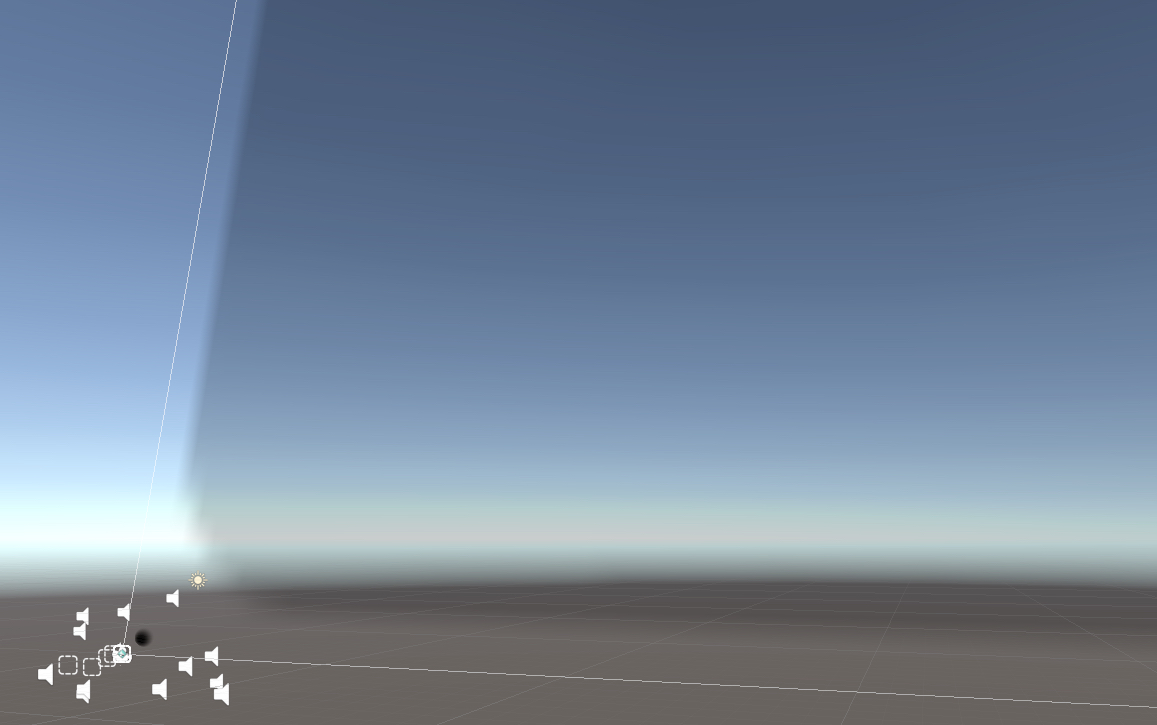
\includegraphics[width=0.8\textwidth]{../../Figures/darkpanel.jpg} 
    \caption{Dark background panel to mimic darkening of the user's visual field} 
    \label{fig:darkpanel} 
\end{figure}

At the start of the simulation, the alpha value of this panel is set to zero, ensuring that the screen appears completely transparent and preventing any initial visual flash. With the start of the simulation a coroutine is triggered that increases the panel’s alpha value from 0 to 0.7 over a duration which can be set in Unity itself, called the (\texttt{fadeDuration}, typically 2 seconds).

The darkening culminates in a panel opacity of 70\% (i.e., \texttt{alpha = 0.7}), which darkens the screen significantly without making it fully dark. This design choice maintains visibility while still inducing a sense of discomfort or visual strain. As such, the effect models subtle visual hallucinations or perceptual narrowing, which are commonly reported in psychotic experiences. 

\subsubsection{Stains}
One effect, created using the \texttt{DynamicWaveDeformation.cs} script, makes the surfaces of objects appear to ripple and shift. This gives them a wavy, moving look that reflects how perception can feel distorted during hallucinations. This deformation was applied to spheres which are triggered by a pre-defined spawn and disappearance interval. The spheres are randomly placed in the user's field of view, and they float around, creating a sense of visual noise. The \texttt{FadeEdgeShader.shader} shader was used to create a darkening effect around the edges of the screen, simulating the feeling of being in a confined space or having a limited field of vision. This shader was created with the help of ChatGPT, which provided a basic structure that was then customized to fit the specific needs of the simulation.

The \texttt{Orchestrator.cs} script manages when these spheres appear during the simulation timeline. The method \texttt{SpawnSphere()} is invoked repeatedly in a loop to instantiate the spheres at randomized positions around a central \texttt{spawnPoint}. The number of spheres and the interval between their appearances are determined by the parameters \texttt{sphereCount} and \texttt{spawnInterval}, respectively.Each sphere is placed within a circular area defined by a \texttt{spawnRadius}, with its Y-coordinate fixed to match the user’s eye level for spatial consistency. After a fixed delay, the spheres are removed in the same order they appeared, one by one, using a queue-based removal mechanism and the \texttt{Destroy()} function. 

\vspace{1em}

The visual appearance of these spheres is designed to be ambiguous and somewhat unnatural. They show a constantly shifting surface that pulses and distorts as if they are made out of a wavy material to represent stains. This is achieved through the \texttt{DynamicWaveDeformation.cs} script, which displaces the vertices of each sphere's mesh in real time, to create this wave effect.

When oinstantiated, the script stores the original mesh vertices and continuously updates them every frame based on the wave function that combines sine and cosine operations on both the X and Z components of each vertex:

\begin{quote}
\texttt{float wave = sin(time + x) * cos(time + z)}
\end{quote}

The wave value is multiplied by a configurable strength parameter called \texttt{waveAmplitude}, and this result is used to slightly move each point on the sphere’s surface outward or inward along its normal direction. This creates a rippling effect across the whole object, making the sphere appear as if it is softly pulsing or "breathing" while it exists in the environment.


\paragraph{Visual Example}
Figure~\ref{fig:stain} shows a black deforming sphere as it appears in the real-world mixed reality classroom context. The shader used for this object includes a soft fade around the edges, giving it a non-solid, ghostly appearance that blends slightly with the background. Figure~\ref{fig:fadeedgeshader} illustrates the same object in the Unity Editor, where the mesh deformation and alpha transparency are more clearly visible.


\begin{figure}[h!] 
    \centering 
    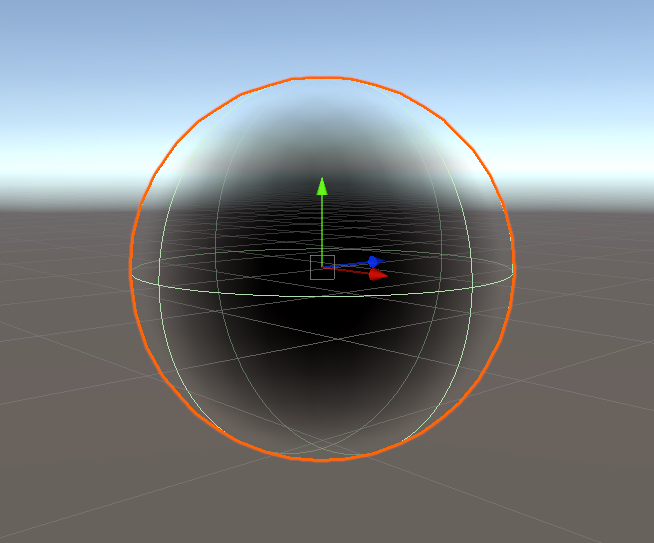
\includegraphics[width=0.6\textwidth]{../../Figures/fadeedgeshader.jpg} 
    \caption{Example sphere with the \texttt{FadeEdgeShader.shader} and the \texttt{DynamicWaveDeformation.cs} script to mimic stains} 
    \label{fig:fadeedgeshader} 
\end{figure}

\begin{figure}[h!] 
    \centering 
    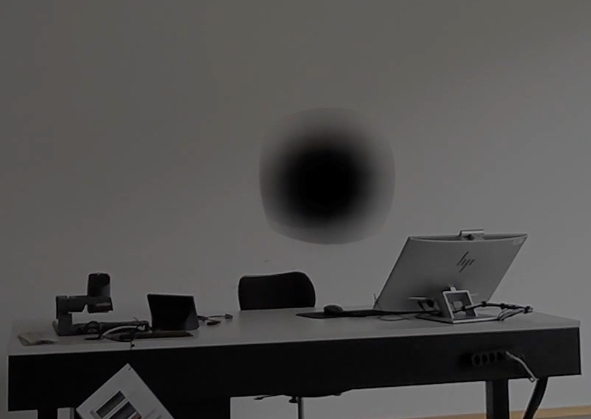
\includegraphics[width=0.6\textwidth]{../../Figures/stain-video.jpg} 
    \caption{Stain appearing in the user's field of view} 
    \label{fig:stain} 
\end{figure}

\subsubsection{Floating Dots and Interaction Logic}

To help simulate the kind of perceptual disturbances that some people with psychosis experience, the simulation includes floating colored dots that the user can interact with. These are controlled by two main scripts: \texttt{DotManager.cs}, which creates the floating dots, and \texttt{ObjectCollision.cs}, which handles what happens when users touch the interactive spheres.

\vspace{1em}

The \texttt{DotManager.cs} script is responsible for filling the space around the user with a number of small red and blue spheres—referred to as “dots.” These dots are placed randomly within a area, defined by the parameters \texttt{spawnWidth}, \texttt{spawnHeight}, and \texttt{spawnDepth}. To not overcrowd the visual field, the script makes sure that each dot is placed far enough away from the others. If a dot would be too close to a previous one, a new position is chosen.

Each dot is randomly colored red or blue, creating a scattered, noisy effect. The idea is to make the environment feel just a bit off or overwhelming, without making it frightening.The dots are also meant to be more interactive. They appear at different moments in the simulation and are set up to respond when the user reaches out and touches them. The logic behind this is handled by the \texttt{ObjectCollision.cs} script.

Using Unity's collision detection system, the script monitors for \texttt{OnTriggerEnter} and \texttt{OnTriggerExit} events. When the user's hand (or other collider) enters the trigger zone of a sphere, the following actions are executed:

\begin{itemize}
    \item The object's material is changed to a new, randomly generated color using \texttt{Random.ColorHSV()}. This signals to the user that the object has responded to their touch.
    \item The script searches the scene for an \texttt{AudioSource} tagged as \texttt{"Audio10"} and stops it using \texttt{audioSource.Stop()}. This source plays a looping sound \textit{"Touche les points !"} (Touch the dots!), intended to mimic intrusive auditory hallucinations. Its termination represents a temporary sense of relief or control.
\end{itemize}

The interaction is simple but meaningful. It represents how some people try to manage or quiet their hallucinations—by focusing on them or interacting in some way. In the simulation, this also makes the experience more engaging and lets users take an active role, rather than just being passive observers.

\paragraph{Visual Example}
The images below illustrate the interaction process. In Figure~\ref{fig:dots_before}, the user sees floating dots in their original red and blue state. After touching a sphere, as shown in Figure~\ref{fig:dots_after}, the affected object changes color, confirming that the interaction was registered and the audio loop was interrupted.

\begin{figure}[H]
    \centering
    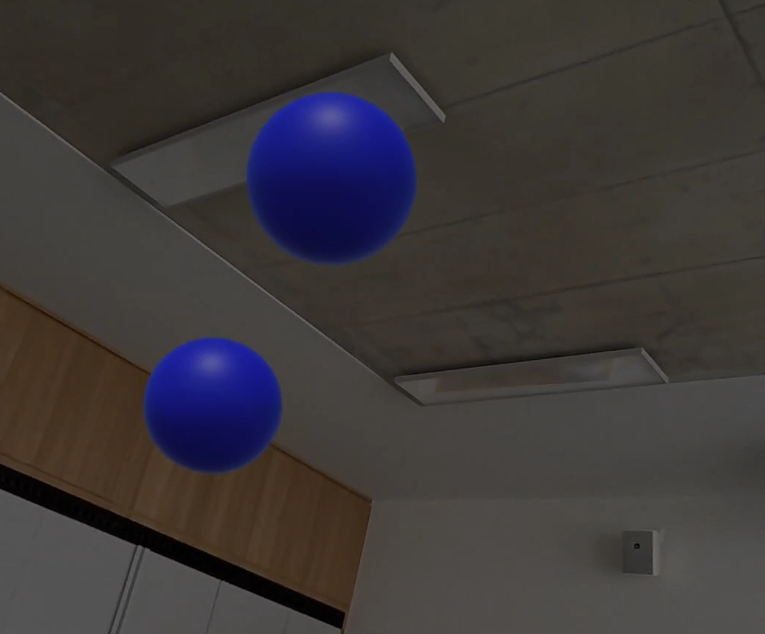
\includegraphics[width=0.6\textwidth]{../../Figures/dots-video.jpg}
    \caption{Floating dots before user interaction.}
    \label{fig:dots_before}
\end{figure}

\begin{figure}[H]
    \centering
    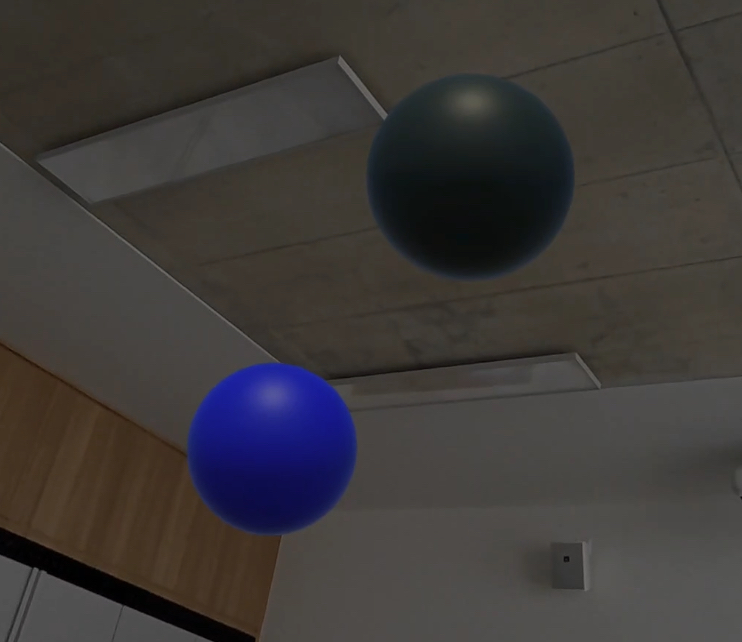
\includegraphics[width=0.6\textwidth]{../../Figures/dots-after-touch.jpg}
    \caption{Color change after user touches one of the dots.}
    \label{fig:dots_after}
\end{figure}


Together, these two systems—floating dots and interactive auditory element of the dots—form a approach to simulating environmental disruption. While the \texttt{DotManager.cs} creates persistent visual distraction, the \texttt{ObjectCollision} system adds intensity. The use of sound looping and the color change of the dots reinforces the themes of intrusion and momentary relief, central to the projects goal of eliciting empathetic insight into the lived experience of a psychosis.


\section{Challenges During Implementation} 
Despite careful planning, several significant challenges emerged during the development of the simulation:

\subsection{Audio Loops} 
Initially, each interactive sphere instantiated its own sound playback. This led to multiple overlapping sound loops, which had to be fixed. The problem arose because the audio logic was not centralized — each sphere's ObjectCollision component independently triggered audio playback upon spawning. For example, if five spheres were instantiated, each would play its own sound, leading to overlapping audio. The audio would then only stop, if all five spheres were touched, which was not the intended behavior.

To solve this issue, a shared audio management system was developed, which is a static AudioSource and coroutine created within \texttt{ObjectCollision.cs}. This means that only one looped sound source exists, and it is globally stopped when a user interacts with any sphere.

A key logic excerpt illustrating this centralization is:

\begin{quote} \small \texttt{if (sharedAudioSource == null) { sharedAudioSource = ...; coroutineHost = this; repeatCoroutine = coroutineHost.StartCoroutine(RepeatAudio());}} \end{quote}

This ensures no duplicate sounds occur, even with multiple spheres present.

\subsection{Finger Interaction} 
A second major challenge was accurately detecting when a user touched a dot. Initially, an additional \textit{poke interaction} module was mistakenly integrated alongside the already built-in collision detection by Unity. This redundant system caused conflicting behavior and unpredictable touch responses. Upon deeper inspection, it was discovered that Unitys hand collision system already assigns specific identifiers to each fingertip collider, such as \textit{HandIndex1} for the index finger. Reliable detection could therefore be implemented simply by checking the collision object's name during a collision event, rather than adding redundant interaction modules.

\begin{quote} \small \texttt{if (collision.gameObject.name.Contains("HandIndex1")) { ... }} \end{quote}

By implementing this and removing the redundant poke interaction, the color changing was a smooth process and the finger identification also worked.

\subsection{Loud Audio} 
During preliminary testing, the built-in speakers of the Meta Quest 3 were found to be too loud, leaking audio to the entire room and were being heard by observers. To address this, PhoneLook bone-conduction headphones\footnote{\url{https://www.phonelook.ch/de/stylische-kabellose-bluetooth-knochenleitungs-kopfhorer-fur-sport-laufen-radfahren-fitness-schwarz.html}} were integrated into the simulation setup. This had the advantage that the audio is transmitted privately to the participant without occluding ambient sounds.
It also ensures immersive simulatin while respecting privacy and the testing environment.

\subsection{Spatial Placement of Audio } 
Another significant challenge was the spatial arrangement of audio sources within the simulation environment. Initially, it was difficult to orient myself correctly in Unityss Scene View, making it unclear where the sounds would originate from relative to the user position. Proper placement was essential to create a convincing spatial auditory experience, because sounds had to feel anchored in specific locations in the environment. As the user moved, the sounds needed to remain fixed in space, enhancing realism and immersion.

To solve this, I invested time to become familiar with Unity's camera controls and 3D scene navigation.Then, the sound sources were distributed strategically across different coordinates, ensuring that different hallucinated voices would come from distinct spatial directions.

An example of the 3D placement of the sound sources in the Unity scene is shown in \autoref{fig:sound_sources}.

\begin{figure}[h!] \centering 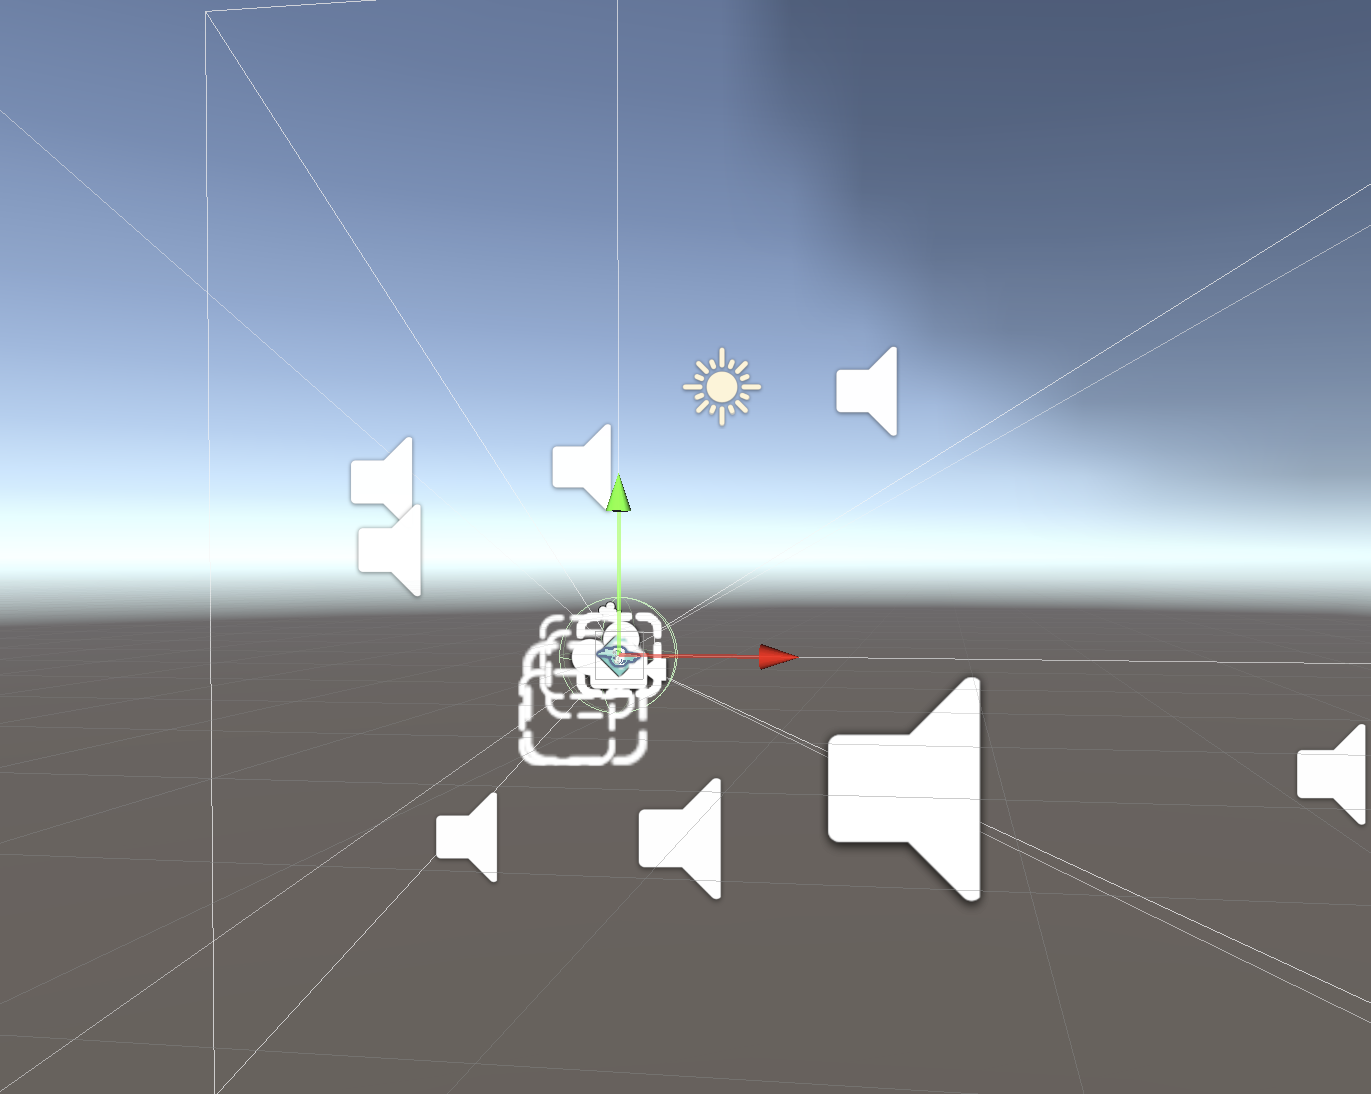
\includegraphics[width=0.8\textwidth]{../../Figures/unity-scene.png} \caption{Placement of spatial sound sources in the Unity scene for the hallucination simulation. Each speaker icon represents a sound source emitting a hallucination voice.} \label{fig:sound_sources} \end{figure}


\newpage{\pagestyle{empty} \cleardoublepage}

\chapter{User Study Design and Methodology}
\label{ch:userstudy}


To systematically evaluate the educational and empathic impact of the MR simulation, a controlled user study was conducted with a total of 29 medical students enrolled at the Haute école de santé Fribourg (HEdS-FR). The study employed a pretest–posttest mixed-methods design, combining quantitative measures with group interaction and reflective feedback to understand the effects of the simulation experience.

\section{Study Design Overview}

The user study followed a three-phase structure: pre-simulation evaluation, simulation experience, and post-simulation evaluation. This structure allowed for a measurement of change in empathy and emotional response, and offered insight into both the direct effects of the MR simulation on the headset user and the indirect effects on observing students. The design aligns with educational best practices and recommendations in empathy training, particularly those emphasizing immersive realism combined with ethical framing and debriefing.
The study was conducted in a controlled environment, with all participants receiving the same information and instructions. The simulation was designed to be brief yet impactful, allowing for a focused exploration of the experience of psychosis while minimizing potential distress.
The study was approved by the HEdS-FR ethics committee, and all participants provided informed consent prior to their involvement. The study was conducted in accordance with ethical guidelines for research involving human subjects, particularly in the context of medical education and simulation.

The evaluation included both quantitative and qualitative components:

\begin{itemize}
  \item \textbf{Pre-Evaluation:} Conducted immediately before the simulation, this questionnaire assessed participants prior experience with patients (especially those diagnosed with schizophrenia), and measured baseline empathy and emotional perceptions.
  \item \textbf{Post-Evaluation:} Completed directly after the simulation, this questionnaire repeated the empathy and emotion assessments and included additional questions about the participants experience with the simulation.
\end{itemize}

Two groups were compared in the post-evaluation: participants who engaged in the simulation as "observers" (without the headset) and those who used the mixed-reality headset individually.

\section{Participants}

The target group for this study consists of medical students in their preclinical or early clinical training, specifically from the University of Health in Fribourg, Switzerland (in French: Haute école de santé Fribourg, HEdS-FR). This population was selected for two primary reasons. First, students at this stage are actively developing their clinical attitudes, including their capacity for empathy toward patients. Second, previous research has shown that empathy training tends to be particularly effective during this formative period in a healthcare professionals education \cite{Hsia2022, Kuhail2022}.

Participation in the study is voluntary, and all participants are recruited through internal communication channels within the university. Before taking part, each participant receives comprehensive information about the objectives of the study, its procedures, and potential risks. They are informed of their rights, including the ability to withdraw at any time, and are asked to sign a written consent form confirming their understanding and agreement.


\section{Procedure}

The study is conducted in small groups. A total of five groups, each consisting of six students, participate in the simulation sessions. Within each group, only one student wears the MR headset and experiences the simulated symptoms. The other five students remain in the room during the simulation and are given a specific task by the instructor. Their role is to observe the behavior of the participant wearing the headset, noting any signs of confusion, distraction, or distress. This setup serves two purposes: first, it mirrors real clinical scenarios where healthcare providers must interpret subtle behavioral cues; and second, it allows researchers to explore whether witnessing someone elses simulated experience can also affect empathy and perception from an external, observational perspective.

All six group members—both the headset user and the observers—complete the same set of questionnaires. These include the Jefferson Scale of Empathy (JSE) \cite{Hojat2002} to assess baseline and post-simulation empathy levels, and the Brief Positive and Negative Affect Schedule (B-PANAS) \cite{Boiroux2024} to measure emotional responses and perceptions toward individuals with schizophrenia. The evaluation process is described in more detail in Chapter~\ref{ch:eval}.

The simulation itself lasts approximately 3 to 4 minutes. During this time, the student wearing the headset is exposed to a carefully sequenced combination of auditory and visual hallucinations, all set within a familiar environment such as a classroom. The goal is to simulate psychotic symptoms in a way that is immersive but safe, and to encourage emotional and cognitive engagement with the experience.

Immediately following the simulation, all group members take part in a structured debriefing session moderated by teaching staff. This guided reflection allows participants to discuss what they observed or experienced, process their emotional responses, and relate the exercise to their future clinical work. For the observers in particular, this provides an opportunity to articulate how witnessing the simulation affected their perception of both the symptoms and the individual undergoing them.

After the debriefing, participants once again complete the JSE and B-PANAS questionnaires to assess any changes in empathy levels and emotional responses. They are also invited to provide qualitative feedback on the simulation, including comments on its realism, emotional impact, and educational value. The inclusion of both direct and indirect participants allows the study to assess how empathy might be influenced not only by immersive first-person experiences, but also through empathetic observation—a dimension that has received limited attention in the literature.


\subsection{JSE and B-PANAS Scales}
\label{ch:eval}
The evaluation of the MR simulation's impact on empathy and emotional response is conducted using two primary measurement tools: the Jefferson Scale of Empathy (JSE) and the Brief Positive and Negative Affect Schedule (B-PANAS). These tools are designed to capture both cognitive and affective dimensions of empathy, as well as emotional responses to individuals with schizophrenia.

\subsubsection{Jefferson Scale of Empathy (JSE)}
\label{sec:jse}

The primary tool used to measure empathy is the Jefferson Scale of Empathy (JSE), which is widely applied in medical education and has been shown to reliably measure both affective and cognitive components of empathy \cite{Hojat2002}. The JSE is administered before and after the MR simulation to assess whether the experience has led to measurable changes in students’ empathy levels. The results are analyzed to determine changes in total empathy scores, as well as shifts in cognitive and affective empathy dimensions.

Since the JSE was originally developed in English and no officially validated French version was available for this study, the questionnaire was translated into French by the researcher using a combination of online translation tools and manual adjustments. While care was taken to preserve the meaning and intent of the original items, this translated version has not undergone formal psychometric validation. As such, the use of this adapted French version represents a methodological limitation and should be considered when interpreting the results.

To better align the measurement tool with the goals of this study—namely, to evaluate both cognitive and affective components of empathy in a balanced and time-sensitive way—the full JSE was thematically reviewed and categorized by the author. Based on an in-depth literature review and the conceptual definitions of empathy used in this thesis, each item was classified as either \textit{Cognitive} or \textit{Affective}. Cognitive items reflect an emphasis on understanding the patient’s perspective, thoughts, or non-verbal cues, while affective items relate to emotional awareness, resonance, or the therapeutic value of emotional understanding. A detailed overview of this classification can be found in Appendix~\ref{app:jse}, Table~\ref{tab:jse_classification}.

In order to maintain engagement, a shortened version of the JSE was developed. This version includes 13 items—five reflecting cognitive empathy and 8 reflecting affective empathy—that were selected based on thematic clarity and their alignment with the measurement goals of the study. The item selection are shown in Appendix~\ref{app:jse-short}, Table~\ref{tab:jse_shortened}. % explain why these items?

\subsubsection{Emotional Response (Positive and Negative Affect)}

To better understand the emotional impact of the simulation, students were asked to rate the intensity of their own emotional responses when thinking specifically about individuals diagnosed with schizophrenia. This part of the questionnaire was adapted from a validated French-language version of the Positive and Negative Affect Schedule (PANAS), as published by Boiroux (2024) \cite{Boiroux2024}. Participants rated each emotion on a 5-point Likert scale ranging from 1 (“Pas du tout” / “Not at all”) to 5 (“Extrêmement” / “Extremely”).

The selection of emotional terms was carefully curated to include an equal balance of five positive and five negative affective states. The goal of this design was to explore how the simulation might shift students’ emotional associations with schizophrenia—either increasing compassionate or empathetic responses, or reducing feelings of fear, anxiety, or social discomfort. Rather than merely recording whether emotions intensified or weakened overall, the approach focused on identifying which specific emotional tones were affected and in what direction.

The following ten emotions were included in the questionnaire:

\begin{quote}
\textit{Angoissé(e) (Anxious), Enthousiaste (Enthusiastic), Honteux(se) (Ashamed), Inspiré(e) (Inspired), Intéressé(e) (Interested), Irrité(e) (Irritated), Craintif(ve) (Fearful), Alerte (Alert), Attentif(ve) (Attentive), and Nerveux(se) (Nervous).}
\end{quote}

This set provides a balanced perspective on affective response. Positive terms such as \textit{enthousiaste}, \textit{inspiré(e)}, and \textit{intéressé(e)} were selected to assess potential increases in empathy, engagement, and curiosity following the simulation. In contrast, negative emotions like \textit{angoissé(e)}, \textit{honteux(se)}, and \textit{craintif(ve)} were included to evaluate whether the experience reduced discomfort, fear, or stigma-related reactions.

This measurement strategy supports a more nuanced understanding of how the MR simulation influenced the emotional lens through which students perceive individuals with schizophrenia. It complements the cognitive and affective empathy data from the JSE by offering insight into the emotional tone behind students’ attitudes—an important factor in building compassionate clinical behavior.


\subsection{Perceptions of the Simulation}

In addition to the JSE and the emotional response, participants which wore the headset, complete a short questionnaire immediately after the simulation, which evaluates their perceptions of the experience. This includes five statements rated on a 7-point Likert scale (1 = “Strongly disagree” to 7 = “Strongly agree”). The items are designed to assess how educational, immersive, and useful the simulation was perceived to be, as well as its potential to increase understanding and empathy. Example items include: \emph{translate to english (?)}

\begin{itemize}
    \item \textit{La simulation était éducative.} \\
    \textit{The simulation was educational.}

    \item \textit{La simulation est un moyen efficace de sensibiliser à la schizophrénie.} \\
    \textit{The simulation is an effective way to raise awareness about schizophrenia.}

    \item \textit{La simulation devrait rendre les gens plus compréhensifs à l’égard des personnes atteintes de schizophrénie.} \\
    \textit{The simulation should help people become more understanding toward individuals with schizophrenia.}
\end{itemize}

This helps evaluate how participants interpreted the experience and whether they found it meaningful in a learning context.

\subsection{Debriefing and Reflection}

Following the simulation and post-questionnaire phase, all participants engaged in a structured debriefing session facilitated by a faculty moderator. This session provided a safe space for emotional and intellectual reflection. Participants were encouraged to share their thoughts, feelings, and interpretations of both the simulation and their observations. The discussion also addressed how the simulation might influence their attitudes or behaviors in future clinical interactions with patients diagnosed with schizophrenia.

\section{Data Collection and Analysis}

The data collected during the user study included both quantitative and qualitative components. Quantitative measures consisted of pre- and post-simulation scores on the JSE and B-PANAS for all participants, as well as Likert-scale responses to the post-simulation perception questionnaire completed by the headset user. These data were analyzed using within-subject comparisons, primarily through paired t-tests, to detect statistically significant changes in empathy and emotional affect. Differences between headset users and observers were also examined to explore how first-person versus observational engagement influenced outcomes.

Qualitative data were derived from transcripts of the debriefing sessions (with participant consent). These responses were analyzed using thematic coding to identify recurring motifs, such as emotional resonance, perceived realism, educational value, ethical reflections, and shifts in attitudes or understanding.

\section{Ethical Considerations}

Given the potentially distressing nature of psychosis simulation, the study was designed with multiple ethical elemnets. Participants received clear pre-study briefings and signed informed consent forms. The simulation was kept short in duration and grounded in a familiar environment to minimize psychological risk. The debriefing session served not only as a pedagogical tool but also as a psychological buffer, ensuring that students could process the experience in a safe, reflective manner. Participants were also reminded of their right to withdraw at any point without consequence.

\section{Summary}

Together, the combination of the JSE, perception ratings, emotional intensity scales, and optional qualitative feedback provides a well-rounded view of the simulation’s effectiveness. This multi-method approach is designed to explore whether a brief MR simulation can positively affect both empathy and emotional understanding, while also providing insights into the simulation’s usability and educational value.


\newpage{\pagestyle{empty} \cleardoublepage}

\chapter{Results and Analysis}
\label{ch:resultsandanalysis}

This chapter presents the results of both the quantitative and qualitative analysis conducted to evaluate the impact of the mixed-reality simulation on participants empathy and emotional responses toward individuals with schizophrenia. It begins with a breakdown of pre-evaluation findings that show baseline attitudes and empathy. Post-evaluation results are then presented, including changes in empathy and emotional states across the full sample, as well as subgroups (group participants and individual headset users). Statistical comparisons are used to assess whether observed differences are significant. Finally, we integrate observational and verbal feedback from participants to complement and contextualize the quantitative data. This mixed-methods approach allows for a richer understanding of the simulationss effects, particularly in areas not captured by standardized measures.

\section{Pre-Evaluation Results}
The pre-evaluation phase was conducted prior to any exposure to the simulation. It served to assess baseline levels of empathy and emotional responses toward individuals with schizophrenia. We also collected information on participants' experiences with patients and with that also patients with schizophrenia, which may influence their perceptions.

\subsection{Experience with Patients and Schizophrenia}

Participants were also asked about their prior experience working with patients in general and specifically with individuals diagnosed with schizophrenia. Responses were recorded on a 5-point scale ranging from 1 (No) to 5 (Yes).


\begin{figure}[H]
    \centering
    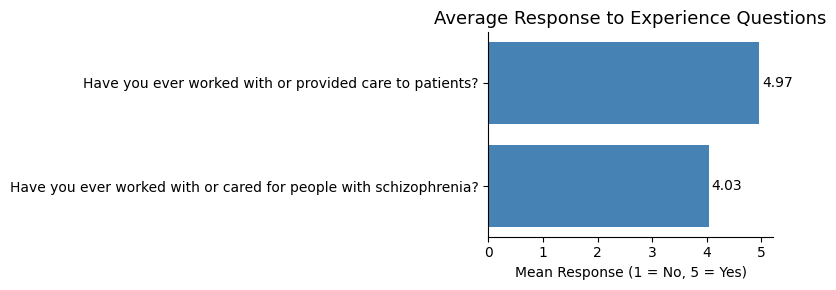
\includegraphics[width=0.7\textwidth]{../../Figures/experience-patients.png}
    \caption{Answers to questions about experience with patients and schizophrenia.}
    \label{fig:experience_patients}
\end{figure}

As shown in Figure~\ref{fig:experience_patients}, nearly all participants reported prior experience working with or caring for patients, with an average response of 4.97. However, fewer had direct experience with individuals with schizophrenia, as indicated by a lower mean score of 4.03. This suggests a general familiarity with healthcare environments, but with that not as much exposure to psychiatric conditions.

\subsection{Baseline Perceptions and Empathy}

Participants responded to a set of 13 Likert-scale items evaluating cognitive and affective components of empathy. These items were scored from 1 (Strongly Disagree) to 6 (Strongly Agree), with reverse scoring applied to negatively phrased statements.

\begin{figure}[H]
    \centering
    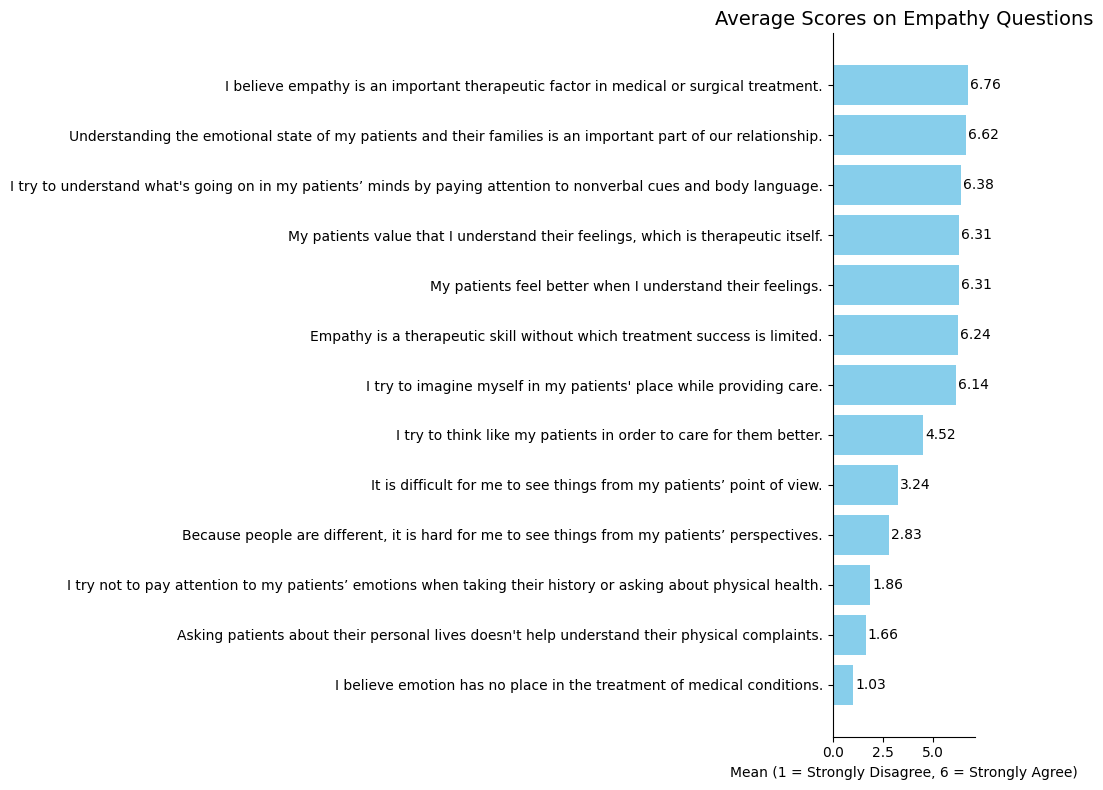
\includegraphics[width=\columnwidth]{../../Figures/avg-scores-pre.png}
    \caption{Average item-wise scores on empathy-related questions.}
    \label{fig:avg_scores_pre}
\end{figure}

Figure~\ref{fig:avg_scores_pre} shows the average scores per item. Responses were generally high for positively phrased statements (e.g., “I believe empathy is an important therapeutic factor”), indicating strong baseline attitudes in favor of empathic engagement. In contrast, negatively phrased items (e.g., “I believe emotion has no place...”) received low agreement, as expected after reverse scoring.

To explore potential variation across groups, empathy scores were also averaged by the time at which participants completed the evaluation session. These groups were constructed based on session start times.

\begin{figure}[H]
    \centering
    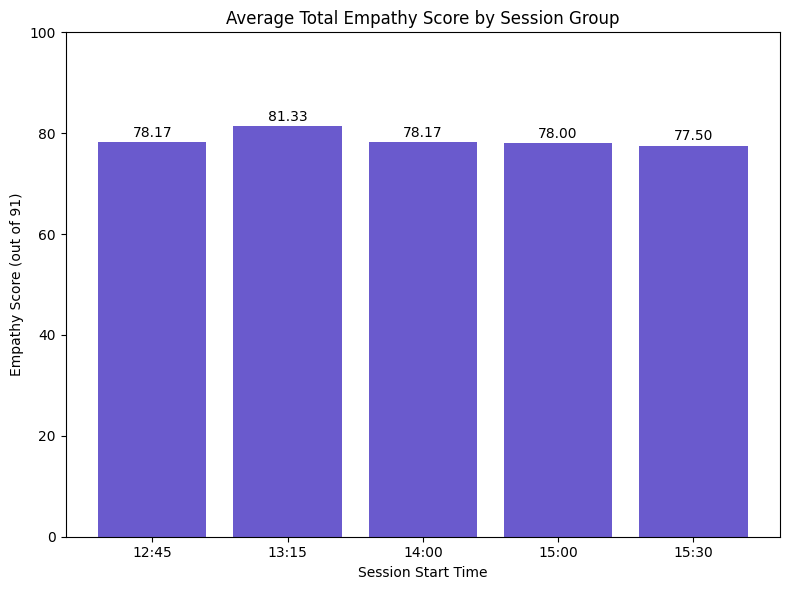
\includegraphics[width=0.75\columnwidth]{../../Figures/avg score-by-group-pre.png}
    \caption{Average total empathy score by session start group.}
    \label{fig:group_scores_pre}
\end{figure}

As shown in Figure~\ref{fig:group_scores_pre}, total empathy scores were relatively consistent across session groups. The highest group average (81.33) was observed for the 13:15 session, though variation across all time slots remained modest (range: 77.50–81.33). This suggests time-of-day or group assignment had minimal influence on baseline empathy.

Participants also rated how strongly they associated various emotions with thinking about individuals with schizophrenia, on a scale from 1 (Not at all) to 5 (Extremely).

\begin{figure}[htbp]
    \centering
    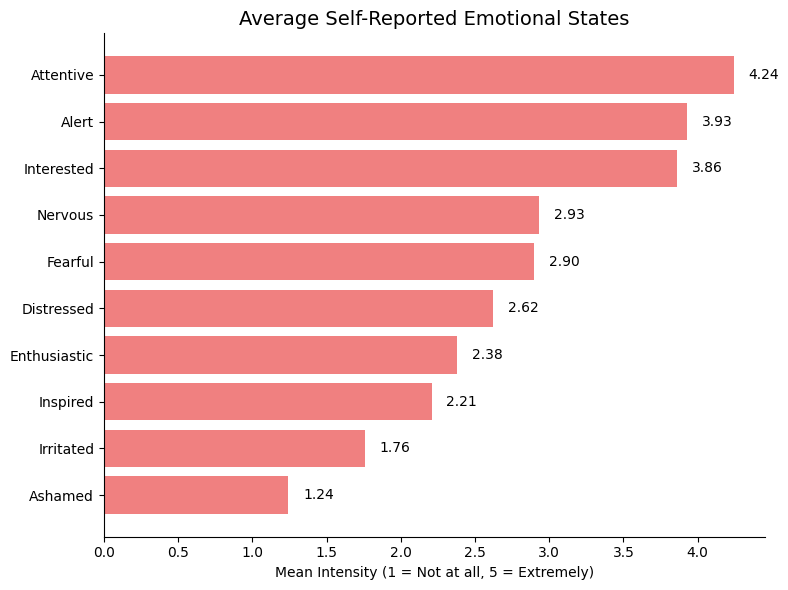
\includegraphics[width=0.7\columnwidth]{../../Figures/avg-emotions-pre.png}
    \caption{Average self-reported emotional intensity associated with thinking about people with schizophrenia.}
    \label{fig:avg_emotions_pre}
\end{figure}

Figure~\ref{fig:avg_emotions_pre} presents the average self-reported intensities for each emotion. “Attentive,” “Alert,” and “Interested” ranked highest, indicating cognitive engagement. Negative emotions such as “Ashamed” and “Irritated” were reported with relatively low intensity, suggesting a limited baseline presence of stigmatizing emotional responses.

\begin{figure}[H]
    \centering
    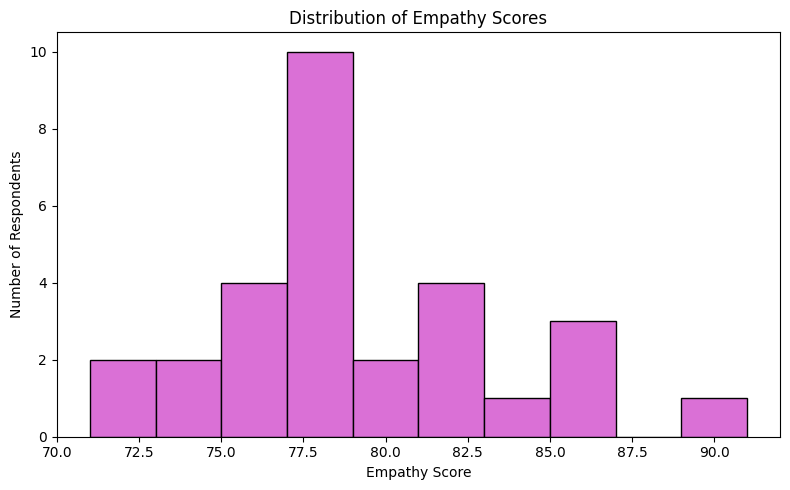
\includegraphics[width=0.75\textwidth]{../../Figures/avg-scores-summary-pre.png}
    \caption{Distribution of total empathy scores among participants.}
    \label{fig:score_distribution_pre}
\end{figure}

Finally, Figure~\ref{fig:score_distribution_pre} displays the distribution of total empathy scores. The majority of participants scored between 75 and 85 out of a maximum of 91, further confirming the high initial level of empathy among the sample.

These baseline findings establish that participants entered the intervention phase with generally high empathy and cognitive openness. This may present a ceiling effect, potentially limiting the observable shift in post-intervention scores.

\section{Post-Evaluation Results}

Following participation in the simulation, participants completed a post-evaluation survey that assessed both their emotional responses and empathy levels, which features the same question set as the pre-evaluation. These include the Jefferson Scale of Empathy (JSE) \cite{Hojat2002} to assess baseline and post-simulation empathy levels, and the Brief Positive and Negative Affect Schedule (B-PANAS) \cite{Boiroux2024} to measure emotional responses and perceptions toward individuals with schizophrenia. This section presents the results for the full sample as well as two subgroups: those who participated in a group setting and those who experienced the mixed-reality (MR) simulation individually using the headset.

Participants were asked to rate the intensity of various emotional states they experienced when thinking about individuals with schizophrenia. These ratings were provided on a 5-point scale ranging from 1 (Not at all) to 5 (Extremely).

\begin{figure}[H]
    \centering
    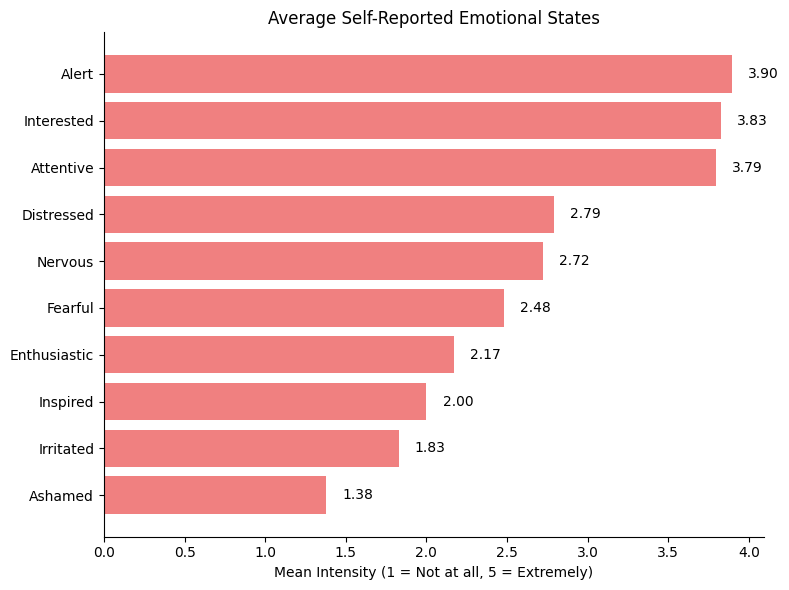
\includegraphics[width=0.75\textwidth]{../../Figures/emotional-post-all.png}
    \caption{Average self-reported emotional states (all participants).}
    \label{fig:emotional_post_all}
\end{figure}

As shown in Figure~\ref{fig:emotional_post_all}, the most intense emotions reported across all participants were \textit{Alert}, \textit{Interested}, and \textit{Attentive}, suggesting a heightened level of engagement and focus during or after the simulation. Emotions such as \textit{Ashamed}, \textit{Irritated}, and \textit{Inspired} were rated much lower, indicating that negative or affectively charged responses were less commonly experienced.

\subsection{Group Participants}

Participants who took part in the simulation in a group setting (e.g., without MR headset) reported emotional responses that were broadly similar to the overall sample. However, their average emotional intensity was slightly higher on items related to awareness and cognitive involvement.

\begin{figure}[H]
    \centering
    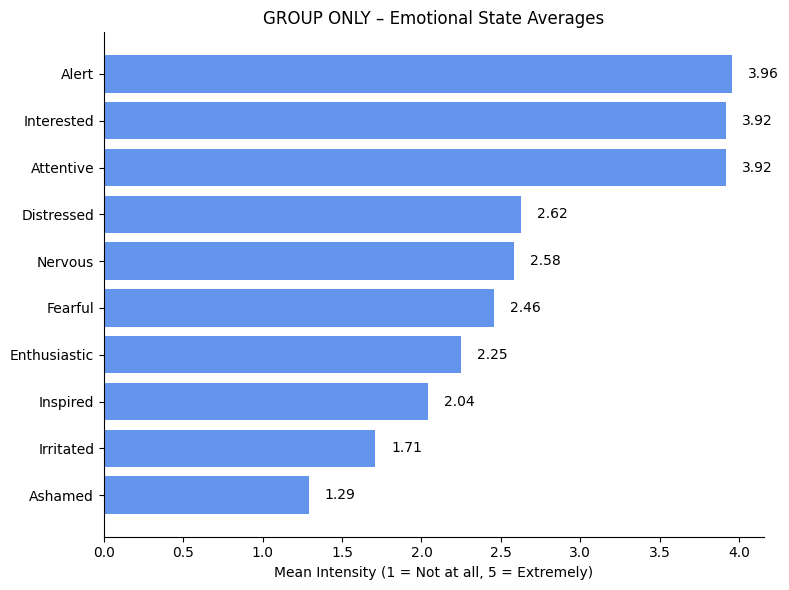
\includegraphics[width=0.75\textwidth]{../../Figures/emotional-post-grp.png}
    \caption{Average emotional state ratings – Group participants only.}
    \label{fig:emotional_post_group}
\end{figure}

As shown in Figure~\ref{fig:emotional_post_group}, \textit{Alert}, \textit{Interested}, and \textit{Attentive} again appeared most strongly. The spread of emotional intensities was relatively consistent with the full group.

The distribution of their overall empathy scores is presented below.

\begin{figure}[H]
    \centering
    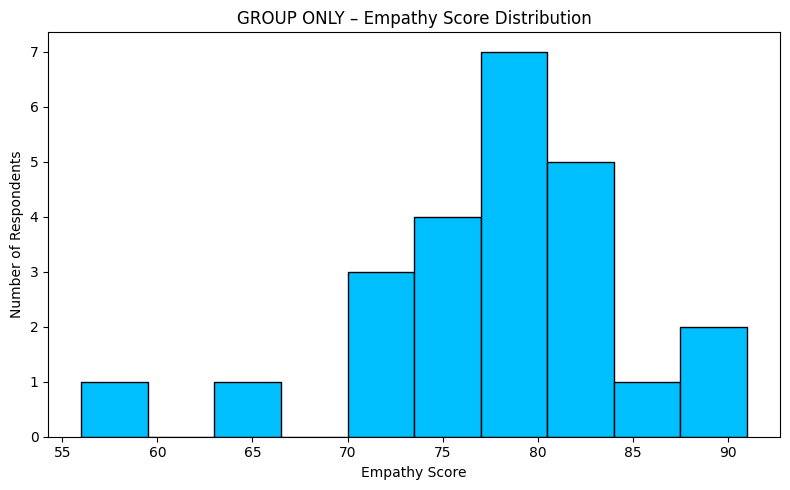
\includegraphics[width=0.75\textwidth]{../../Figures/empathy-score-post-grp.png}
    \caption{Empathy score distribution – Group participants only.}
    \label{fig:empathy_group_post}
\end{figure}

The majority of participants in the group condition scored between 75 and 85 on the empathy scale (max = 91), indicating high levels of empathy across the group.

\subsection{Individual Participants – MR Headset Users}

Participants who engaged with the MR simulation individually using the headset demonstrated slightly different patterns. Their emotional responses included relatively higher levels of \textit{Distress} and \textit{Nervousness}, suggesting a deeper affective impact.

\begin{figure}[H]
    \centering
    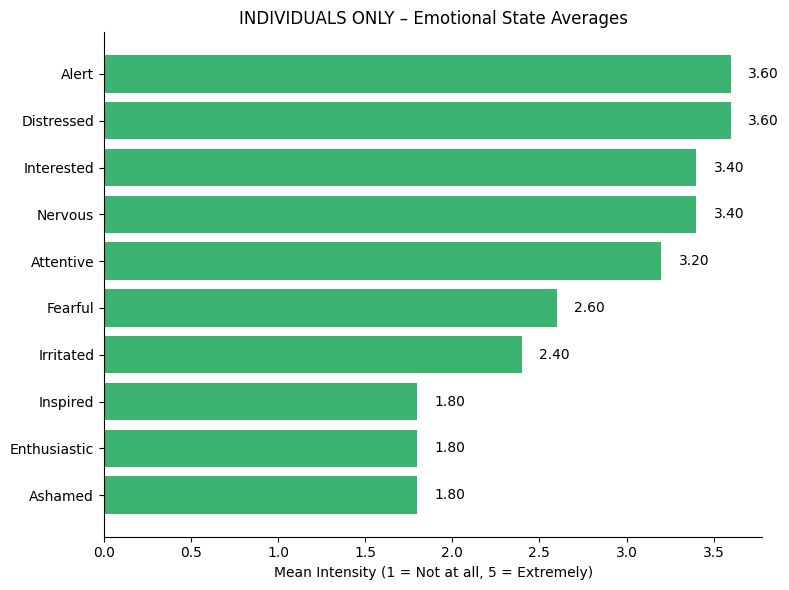
\includegraphics[width=0.75\textwidth]{../../Figures/emotional-post-indiv.png}
    \caption{Average emotional state ratings – Individual (headset) participants.}
    \label{fig:emotional_post_indiv}
\end{figure}

While cognitive engagement emotions like \textit{Alert} and \textit{Interested} remained high, headset users also showed increased ratings for affective states such as \textit{Distressed}, \textit{Fearful}, and \textit{Nervous}, suggesting that the immersive simulation may have elicited stronger emotional reactions.

\begin{figure}[H]
    \centering
    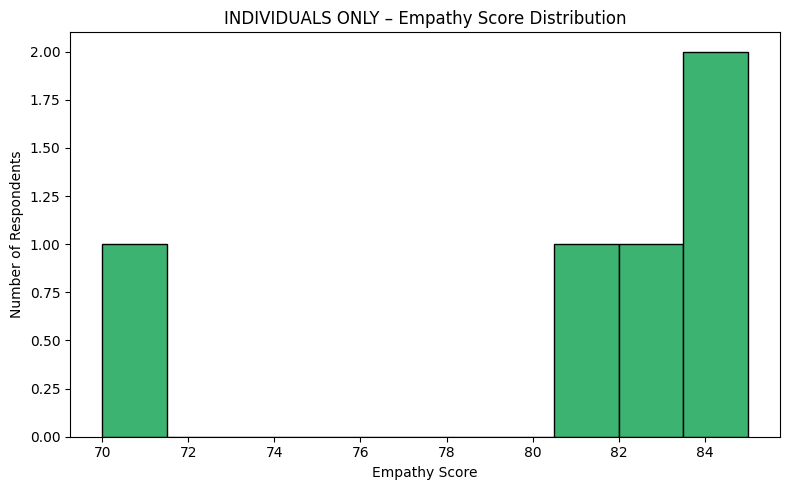
\includegraphics[width=0.75\textwidth]{../../Figures/empathy-score-post-indiv.png}
    \caption{Empathy score distribution – Individual (headset) participants.}
    \label{fig:empathy_indiv_post}
\end{figure}

Empathy scores in this group were tightly clustered at the higher end of the scale, indicating that most headset users reported strong empathic attitudes following the simulation.

\subsection{Overall Empathy Score Distribution}

The full sample distribution of post-evaluation empathy scores is shown below. The majority of respondents scored between 75 and 85 out of 91, reflecting high baseline and post-intervention empathy.

\begin{figure}[H]
    \centering
    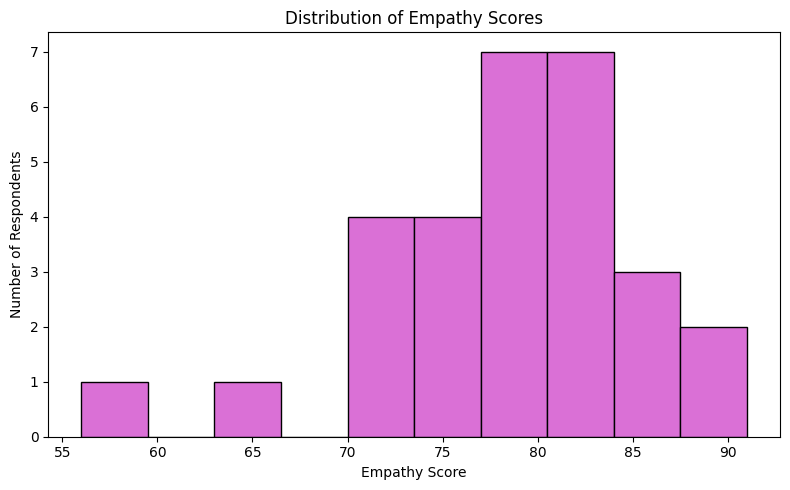
\includegraphics[width=0.75\textwidth]{../../Figures/empathy-score-post-all.png}
    \caption{Empathy score distribution – All participants.}
    \label{fig:empathy_all_post}
\end{figure}

\subsection{Simulation Evaluation Statements}

Participants were also asked to rate their agreement with various statements evaluating the simulation experience. These were scored on a 7-point scale (1 = Strongly Disagree, 7 = Strongly Agree).

\begin{figure}[H]
    \centering
    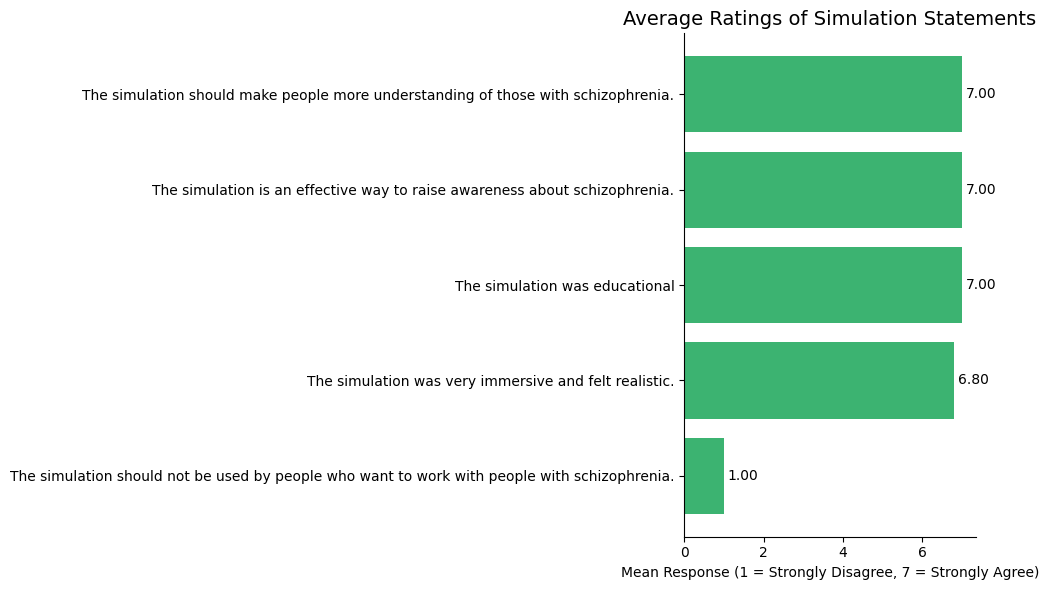
\includegraphics[width=0.9\textwidth]{../../Figures/simulation-evaluation-post.png}
    \caption{Average participant ratings of simulation statements.}
    \label{fig:simulation_evaluation_post}
\end{figure}

Figure~\ref{fig:simulation_evaluation_post} shows near-universal agreement on the simulation’s educational value, realism, and ability to foster understanding. The only statement that received strong disagreement was the suggestion that the simulation “should not be used by people who want to work with people with schizophrenia,” reflecting strong perceived value and acceptability of the tool.

\section{Pre vs. Post Comparison Analysis}
This section presents a statistical comparison of participants’ empathy and emotional responses before and after the simulation experience. By analyzing both group-level changes and individual-level changes, we evaluate whether the intervention led to measurable shifts in perspective or affect. Empathy scores, cognitive and affective, and emotion ratings were analyzed using methods suited for this data.

\subsection{Score Matching and Methodology}

Empathy scores were calculated based on 13 Likert-style attitude items, some of which were reverse-scored to account for negatively phrased statements. Each participant's total empathy score was the sum of their responses, yielding a possible range of 13 to 91 points.

To evaluate changes in emotional response and empathy after the intervention, we conducted paired comparisons between pre- and post-evaluation data. The primary statistical test which was employed for this is the \textbf{Wilcoxon Signed-Rank Test:} used to assess empathetic and emotion-related changes, due to the ordinal nature of Likert data and lack of distribution assumptions.

All tests were two-tailed with a significance threshold of $p < 0.05$. The Wilcoxon test was chosen over a paired t-test due to the non-normal distribution of the data. This approach is robust for small sample sizes and ordinal data \cite{Wilcoxon2013}.

The hypotheses for this test were defined as follows:

\begin{itemize}
  \item \textbf{Null hypothesis ($H_0$):} There is no difference in median empathy scores between the pre- and post-evaluation.
  \item \textbf{Alternative hypothesis ($H_1$):} There is a difference in median empathy scores between the pre- and post-evaluation.
\end{itemize}


\subsection{Statistical Test Results}

To assess the impact of the intervention, we applied statistical tests to compare pre- and post-evaluation responses. These analyses focused on total empathy scores, cognitive and affective empathy subscores, and emotion ratings, with significance evaluated at $p < 0.05$.


\subsubsection{Empathy Score Comparison}

We compared pre- and post-evaluation empathy scores using a Wilcoxon signed-rank test to assess the effect of the intervention.

\begin{itemize}
  \item \textbf{Mean (Pre-Evaluation):} 78.66
  \item \textbf{Mean (Post-Evaluation):} 78.28
  \item \textbf{Wilcoxon test:} $W = 186.0,\ p = 0.7723$
\end{itemize}

While the mean empathy score decreased slightly from pre to post evaluation, the difference was not statistically significant based on either test. The Wilcoxon test returned a p-value of 0.7723, which is well above the common significance threshold of $\alpha = 0.05$. Therefore, we fail to reject the null hypothesis. While the mean empathy score decreased slightly from pre to post evaluation, the difference was not statistically significant. This suggests that the intervention may not have produced a measurable change in empathy, or that individual effects varied too widely for an overall trend to emerge.


\begin{center}
\begin{tabular}{|c|c|c|}
\hline
\textbf{Metric} & \textbf{Pre} & \textbf{Post} \\
\hline
Mean Score & 78.66 & 78.28 \\
Standard Deviation & 4.44 & 7.07 \\
\hline
\end{tabular}
\end{center}

To further explore the effect of the intervention on participant empathy, we examined both the distribution of empathy scores and individual-level changes from pre- to post-evaluation.

\begin{figure}[htbp]
    \centering
    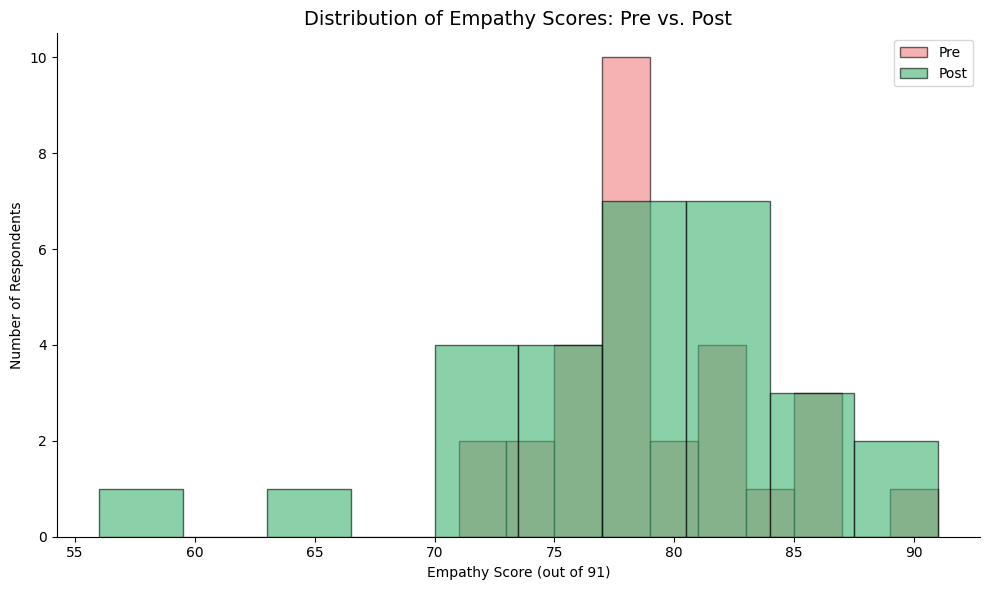
\includegraphics[width=0.75\textwidth]{../../Figures/emp-comparison.png}
    \caption{Distribution of Empathy Scores Before and After the simulation.}
    \label{fig:empathy_dist_hist}
\end{figure}

Figure~\ref{fig:empathy_dist_hist} shows the histogram of empathy scores from the pre- and post-evaluation phases. The distributions are visually similar, with most scores falling between 70 and 85. The post-evaluation scores exhibit slightly more variability, including a small number of lower scores. However, there is also a subtle rightward shift in the upper end, indicating some participants may have increased their scores. Overall, no major distributional shift is apparent.

\begin{figure}[htbp]
    \centering
    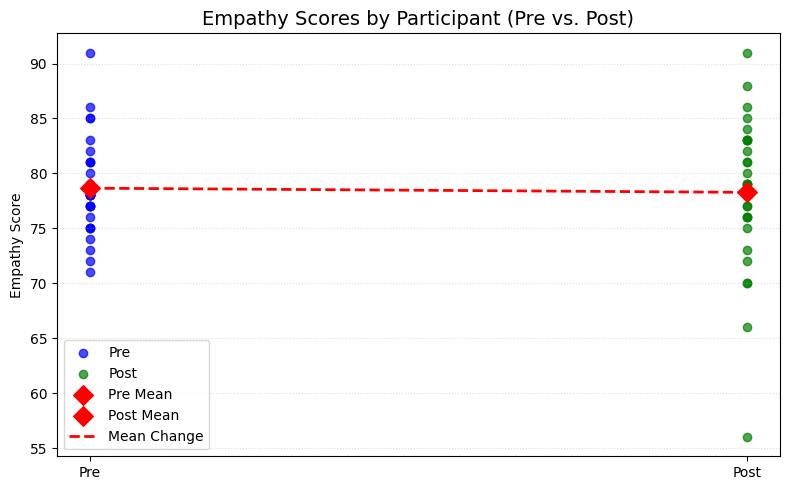
\includegraphics[width=0.75\textwidth]{../../Figures/emph-comparison-means.png}
    \caption{Empathy Scores by Participant: Pre vs. Post with Mean Comparison.}
    \label{fig:empathy_means_line}
\end{figure}

\vspace{1em}

In Figure~\ref{fig:empathy_means_line}, each dot represents a participant’s empathy score before and after the intervention. Red diamonds indicate the group means, and the dashed red line connects the mean pre- and post-scores.

This visualization confirms that although the individual scores are distributed across a similar range, the group mean remained effectively stable. A few participants show noticeable changes in either direction, but the majority maintained consistent empathy scores. The mean dropped slightly from 78.66 (pre) to 78.28 (post), as also reflected in the results of the Wilcoxon signed-rank test ($p = 0.7723$). This supports the interpretation that the intervention did not result in a statistically significant change in overall empathy levels.

\vspace{1em}

These graphs underscore the importance of looking beyond averages: while the group-level effect was minimal, some individuals experienced increases or decreases that could be explored further—especially through qualitative methods or subgroup analysis.

To explore possible group-level effects, we compared average empathy scores by session group. This analysis was motivated by observations made during the simulation sessions: in some groups, the participant using the headset exhibited noticeable engagement — through verbal reactions, physical responses, or expressions of immersion — while in others, the headset user remained relatively passive. Given that the design of the simulation aimed to stimulate empathy through this shared experience, we hypothesized that such variability in engagement might influence group-level outcomes.


\begin{figure}[htbp]
    \centering
    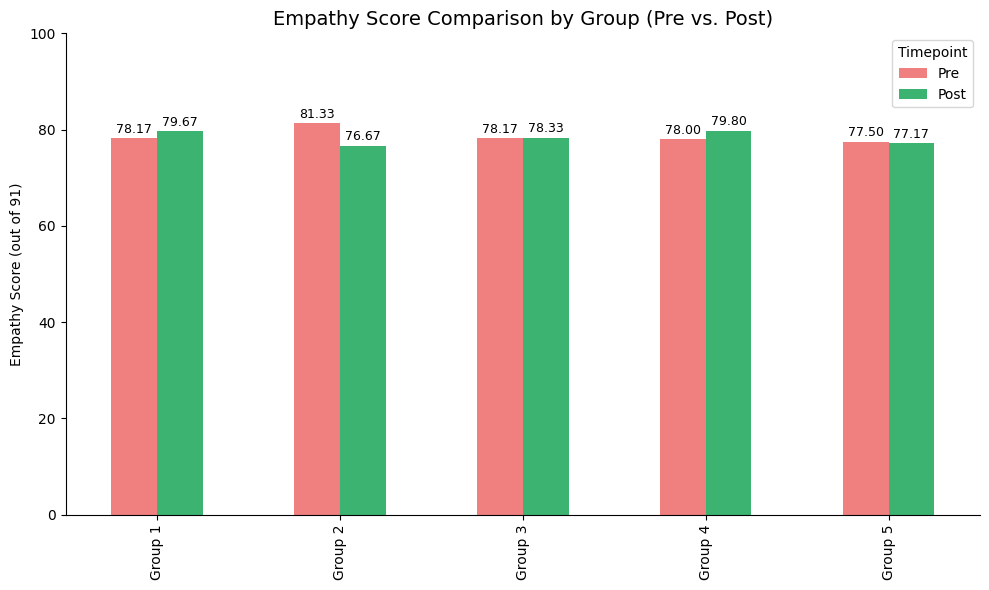
\includegraphics[width=0.85\textwidth]{../../Figures/emph-scores-comp-grp.png}
    \caption{Empathy Score Comparison by Group (Pre vs. Post).}
    \label{fig:empathy_group_bar}
\end{figure}

Figure~\ref{fig:empathy_group_bar} illustrates mean empathy scores for each group before and after the intervention. The scores remain remarkably stable across all groups, with small increases observed in Groups 1, 3, and 4, and small decreases in Groups 2 and 5. None of these differences were large enough to suggest a meaningful group-specific effect. This reinforces the previous conclusion that the intervention did not produce a systematic shift in overall empathy scores.

\vspace{1em}

To better understand the nature of the empathy being measured, the total score is into two subcomponents: \textit{cognitive empathy}, which reflects perspective-taking and understanding mental states; and \textit{affective empathy}, which involves emotional resonance and compassion.

\begin{figure}[htbp]
    \centering
    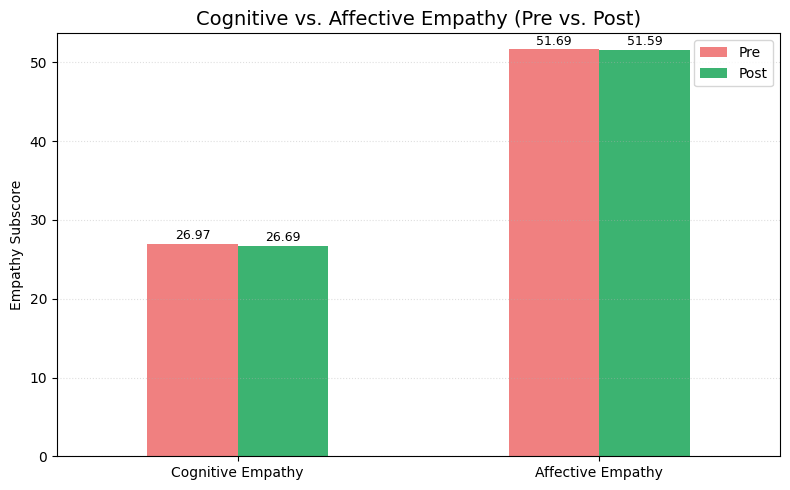
\includegraphics[width=0.75\textwidth]{../../Figures/cog-vs-affect.png}
    \caption{Cognitive vs. Affective Empathy Scores (Pre vs. Post).}
    \label{fig:empathy_cog_aff}
\end{figure}

As shown in Figure~\ref{fig:empathy_cog_aff}, there was almost no change in either subscore. The average cognitive empathy score dropped minimally from 26.97 to 26.69, while the affective empathy score showed an equally small decrease from 51.69 to 51.59. These results suggest that neither cognitive nor affective dimensions of empathy were meaningfully altered by the simulation experience.

Together with the individual, group, and total score analyses, this subscale breakdown adds further support to the interpretation that the intervention had limited impact on participants' self-reported empathy levels — at least as measured immediately after the experience.

% \subsection{Comparison: Individual Headset Users vs. Pre-Evaluation Group}

% To assess whether the most immersive condition—the individual use of the MR headset—was associated with greater empathy, we conducted an exploratory comparison between the post-evaluation scores of headset users ($n=5$) and the pre-evaluation scores of the full participant group ($n=29$).

% The average empathy score for headset users was slightly higher (80.6) than that of the pre-evaluation group (78.7). To test whether this difference was statistically meaningful, we applied the Mann–Whitney U test, a non-parametric method appropriate for comparing two independent groups.

% \begin{itemize}
%   \item \textbf{Mean (Pre-Evaluation Group):} 78.66
%   \item \textbf{Mean (Individual Headset Users):} 80.60
%   \item \textbf{Mann–Whitney U test:} $U = 48.0,\ p = 0.2409$
% \end{itemize}

% As the p-value exceeds the conventional significance threshold of $0.05$, we fail to reject the null hypothesis and conclude that the observed difference is not statistically significant. Nevertheless, the direction of the effect—higher empathy among headset users—may suggest a potential trend.

% \begin{figure}[htbp]
%     \centering
%     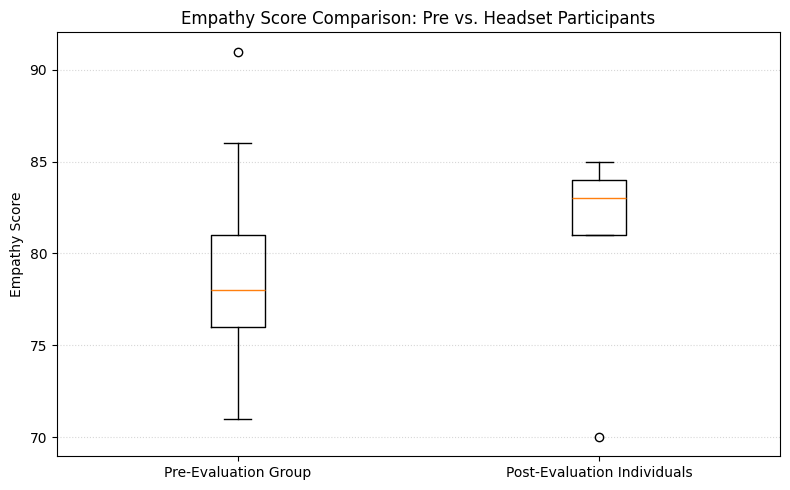
\includegraphics[width=0.75\textwidth]{../../Figures/boxplot-indiv.png} 
%     \caption{Empathy score comparison between individual headset users and pre-evaluation group.}
%     \label{fig:boxplot_indiv_vs_pre}
% \end{figure}

% Given the very small sample size of the individual condition, these results should be interpreted cautiously. However, they offer a potentially meaningful signal: the immersive, embodied experience may have contributed to slightly elevated empathic responses. Future studies should explore this with larger samples and through the integration of qualitative data on individual experiences.


\subsubsection{Emotional Response Comparison}

To explore whether participants’ emotional responses toward people with schizophrenia changed following the simulation, we conducted a series of Wilcoxon signed-rank tests—one for each of the ten emotion items reported pre- and post-intervention.

\paragraph{Hypotheses.} For each emotion, the test was conducted under the following hypotheses:
\begin{itemize}
    \item \textbf{Null Hypothesis ($H_0$):} There is no median difference in emotional intensity pre- and post-simulation; i.e., the simulation did not affect how strongly participants felt the emotion.
    \item \textbf{Alternative Hypothesis ($H_1$):} There is a median difference in emotional intensity between pre- and post-simulation responses.
\end{itemize}

\begin{table}[H]
\centering
\caption{Wilcoxon Signed-Rank Test Results for Emotion Changes}
\begin{tabular}{|l|c|c|c|c|c|}
\hline
\textbf{Emotion} & \textbf{Pre Mean} & \textbf{Post Mean} & \textbf{W-statistic} & \textbf{p-value} & \textbf{Significant} \\
\hline
Attentive     & 4.241 & 3.793 & 72.0  & 0.0633  & False \\
Fearful       & 2.897 & 2.483 & 77.0  & 0.1739  & False \\
Ashamed       & 1.241 & 1.379 & 14.5  & 0.3302  & False \\
Enthusiastic  & 2.379 & 2.172 & 97.5  & 0.3353  & False \\
Nervous       & 2.931 & 2.724 & 86.0  & 0.4702  & False \\
Inspired      & 2.207 & 2.000 & 48.0  & 0.4903  & False \\
Distressed    & 2.621 & 2.793 & 108.0 & 0.5387  & False \\
Irritated     & 1.759 & 1.828 & 47.5  & 0.7483  & False \\
Interested    & 3.862 & 3.828 & 89.5  & 0.8190  & False \\
Alert         & 3.931 & 3.897 & 150.0 & 1.0000  & False \\
\hline
\end{tabular}
\label{tab:wilcoxon_emotions}
\end{table}

None of the tested emotions showed a statistically significant difference between the pre- and post-evaluations at the $p < 0.05$ threshold. The emotion \textit{Attentive} approached significance ($p = 0.0633$), suggesting a possible decrease in attentiveness after the simulation, but this trend did not reach statistical reliability.

To visualize the direction and relative magnitude of changes, the figure below shows the average change in each emotion (post minus pre). Positive values indicate increased emotional intensity post-simulation.


\begin{figure}[H]
    \centering
    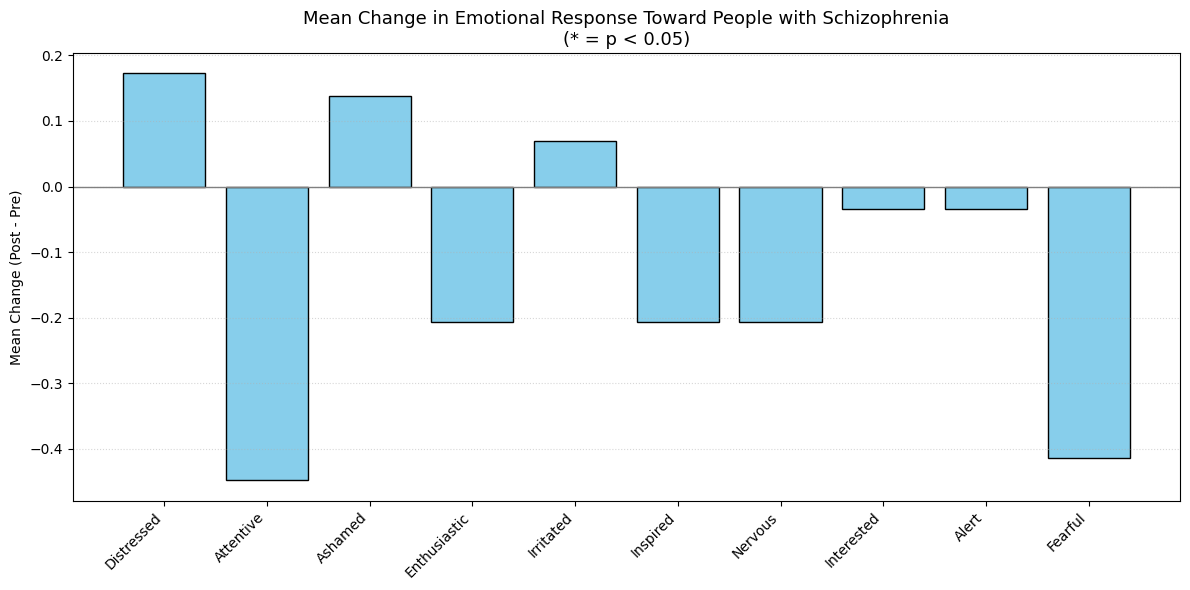
\includegraphics[width=0.85\textwidth]{../../Figures/mean-change-emotions.png}
    \caption{Mean change in emotional response toward individuals with schizophrenia. (* = $p < 0.05$)}
    \label{fig:emotion_change}
\end{figure}

While no statistically significant changes were found, the figure illustrates trends in participants’ emotional shifts. Notably, small increases were observed for emotions like \textit{Distressed}, \textit{Ashamed}, and \textit{Irritated}, whereas emotions such as \textit{Fearful}, \textit{Alert}, and \textit{Attentive} showed modest decreases.

These results suggest that while the simulation may have had subjective effects on emotional perception, the changes were neither strong nor consistent enough to yield significant results across the group. Further qualitative analysis or larger samples may help better characterize individual emotional impacts.


\section{Mixed Methods Integration}
In addition to statistical analyses, observational and self-reported qualitative data were collected to complement the quantitative findings. This included behavioral observations during the MR experience, informal comments post-session, and open-ended feedback where available.

Participants who wore the MR headset shared reflections that contextualized their Likert-scale responses. These insights helped explain individual variability and added depth to our understanding of the simulations emotional impact.


\subsection{Participant Experience and Observational Feedback}

During each session, one participant wore the MR headset simulating auditory and visual hallucinations while attempting to complete a simple task. The rest of the group observed and participated in the same task under normal conditions. This design aimed to allow both the headset user to experience symptoms first-hand and the group to witness their visible effects, ideally fostering empathy through both perspectives.

Notable behavioral patterns varied across participants. Some headset users displayed visible signs of discomfort, such as pinching their lips, turning their heads, hesitating, or seeking clarification. Others remained largely focused on the task, displaying minimal reaction to the simulation.

Group reactions also varied: in some cases, there were uneasy chuckles, concerned glances, or verbal encouragements (“be brave,” “do you need help?”). In other groups, external participants were largely unaware of the internal struggle the headset user was experiencing—sometimes forgetting the headset was even present.

\begin{table}[H]
\centering
\caption{Summary of Headset User Experience and Group Reactions}
\begin{tabular}{|c|p{4.2cm}|p{4.2cm}|p{4.8cm}|}
\hline
\textbf{Group} & \textbf{Headset User Behavior} & \textbf{Group Reaction} & \textbf{Key Participant Quotes} \\
\hline
Group 1 & Nervous laughter, looked around, avoided interacting with virtual elements, reported confusion. & Limited group reaction; one participant quietly offered encouragement. & “The voices keep pulling you down.” \newline “It’s persecution.” \newline “I now understand my cousin better.” \\
\hline
Group 2 & Initially unreactive, later visibly overwhelmed, touched spheres, slight disorientation. & Mild group curiosity, one noted concern, most forgot headset was active. & “There was too much information.” \newline “I forgot the instructions.” \newline “It's harder not to do what the voices say.” \\
\hline
Group 3 & Visibly uncomfortable, delayed task start, repeated lip-pinching, eventually emotional. & Group unaware during task, visibly moved after, discussion emerged post-experience. & “It was horrible.” \newline “I couldn't concentrate... even now I don't know.” \newline “If 2 minutes is absorbing, I can't imagine the people who feel that way every day.” \\
\hline
Group 4 & Focused externally, but no interaction with visual stimuli. Seemed shocked post-experience. & Participant’s distress was internalized; group noticed little during the task. Two members heard audio leaks. & “The voices were disturbing.” \newline “Living the symptoms is another level of experience.” \newline “I think I have more empathy now.” \\

\hline
Group 5 & Started quickly but showed signs of discomfort; pinched lips and waited impatiently for the end. & Group was mostly unaware of the participant’s inner struggle. & “It took a lot of energy and concentration.” \newline “The longer it took, the more frightening it became.” \newline “The simulation helped me realize what they go through.” \\

\hline
\end{tabular}
\label{tab:qual_summary}
\end{table}


\subsubsection{Verbal Feedback from Participants}

Several headset users described strong emotional and cognitive impacts during the debrief. Themes included difficulty concentrating, feeling overwhelmed, dissonance between task instructions and intrusive voices, and a greater understanding of what people with schizophrenia might endure. Some illustrative quotes include:

\begin{itemize}
  \item “We try to focus on something good but the voices keep pulling you down.”
  \item “At first I really didn't want to listen to the voices, but then I couldn't… It's harder not to do what the voices say.”
  \item “I couldn’t understand the instructions… even now I don’t know what we were supposed to do.”
  \item “It was horrible. The voices made simple tasks feel impossible.”
  \item “It was emotionally sad… I didn’t want to look up because I was scared of what I’d see.”
  \item “It took a lot of concentration… I was glad when it was over.”
  \item “I remember my cousin has schizophrenia… now I feel like I better understand what he feels.”
\end{itemize}

Observers also shared reflections:

\begin{itemize}
  \item “I forgot she was wearing the headset… then I saw her moving strangely and I got worried.”
  \item “Seeing her struggle was emotional. It changed how I think about people with schizophrenia.”
  \item “She didn’t react much, so I didn’t realize it was hard for her.”
\end{itemize}

\subsubsection{Interpretation and Reflection}

The qualitative data collected from the debriefs offer valuable insights that contextualize the lack of statistically significant changes in empathy scores. While numeric measures showed minimal change, many participants described deep emotional and cognitive disruption during the simulation, often in ways that are not easily quantifiable.

A consistent theme was the intensity of auditory hallucinations, often overpowering both the visual distortions and the task instructions. Participants reported being distracted, misled, or emotionally shaken. Several remarked on a change in their perspective, noting a greater sense of empathy or awareness after the experience.

\vspace{1em}

Importantly, the visibility of the experience to observers varied greatly. In some groups, the headset users reactions were subtle or absent, making it difficult for others to relate or engage. In others, discomfort or confusion was clearly visible and provoked emotional reactions among the others. This variation highlights the importance of guided debriefs and shared reflection to fully activate the empathy potential of such simulations.

While the intervention may not have uniformly altered self-reported empathy scores, these qualitative accounts suggest that for many participants, the experience was personally impactful—emotionally and cognitively. Future iterations of this intervention may benefit from including structured reflective discussions or journaling to better capture and reinforce these internal shifts.


\section{Summary of Key Findings}

The results of this mixed-methods study suggest that while the MR simulation did not produce statistically significant changes in empathy scores across the entire sample, it nevertheless produced meaningful cognitive and emotional engagement for many participants. Pre-evaluation results indicated that students began the intervention with relatively high levels of empathy and attentiveness, leaving limited room for  movement in quantitative scores—a classic ceiling effect. This was particularly evident in the Jefferson Scale of Empathy (JSE), where most participants scored in the upper range both before and after the simulation.

\vspace{1em}

Post-evaluation data confirmed that self-reported empathy remained largely stable. Neither the total empathy scores nor the subcomponents of cognitive and affective empathy showed significant change following the simulation, and statistical comparisons (Wilcoxon signed-rank test) did not support the hypothesis of a group-level shift. Similarly, emotional affect scores from the B-PANAS showed only modest variation pre- and post-intervention, with none reaching statistical significance. Despite these findings, certain trends were observed, such as a slight decrease in attentiveness and modest increases in distress-related emotions for headset users, hinting at subtle internal shifts not fully captured by the quantitative instruments.

\vspace{1em}

More revealing were the qualitative findings, which offered contextual insight into participants experiences. Headset users frequently described strong emotional reactions to the simulation, including difficulty focusing, feelings of helplessness and emotional discomfort. Many noted that the experience altered how they viewed people living with schizophrenia, leading to greater compassion and understanding. Observers, while less emotionally impacted, also reported increased awareness—particularly when they noticed visible signs of struggle in the headset user.

The simulation was broadly perceived as educational and realistic, with participants agreeing that it helped raise awareness about schizophrenia and could be valuable for those preparing to work in mental health care. In almost all groups, students expressed a desire to reflect more deeply on the experience, particularly during the structured debriefs. These reflections helped surface emotional and empathetic responses that were not always visible in the pre/post metrics but nevertheless shaped their learning.

\vspace{1em}

In summary, the mixed-reality simulation appears to have fulfilled its educational intent by invoking a  personal reflection and generating affective resonance, especially among those who engaged directly with the headset. While the immediate quantitative results were not statistically significant, the qualitative accounts indicate that the simulation meaningfully influenced individual perceptions.
\newpage{\pagestyle{empty} \cleardoublepage}

\chapter{Discussion}
\label{ch:discussion}

\emph{In this section, you should discuss your result and your work. Summarize and discuss your results,  discuss your initial choices and compare with other works from the state of the art. How do you compare (if you can) ? Discuss your research questions in the light of your results. }



\subsection{Interpretation of Changes}

commentary on findings, potential explanations for lack or presence of effect, consideration of variability among participants, comment on potential improvements


While no significant change was observed in the overall empathy score, subtle shifts were detected in emotion-specific responses. For example, participants reported feeling slightly more “distressed” and less “ashamed” when thinking about individuals with schizophrenia post-intervention. However, these changes were not statistically robust in this sample.

Several possible explanations exist:
\begin{itemize}
  \item A \textbf{ceiling effect} may have limited sensitivity, as pre-evaluation empathy scores were already high.
  \item The \textbf{short duration} between evaluations may not have allowed deeper attitude changes to form.
  \item Emotional responses may be more \textbf{situational or reactive} and less stable than overall empathy attitudes.
\end{itemize}

Further qualitative feedback could provide richer insight into participant experiences.


they did not look up for their task, which we should've forced a bit more,
we don't know for sure if we are portraying the experience in a truthful way,
they reported that they felt ashamed to move their hands to be judged by their peers,
they were not able to focus on the task, which is a good thing, but we should've forced them to look up more often,
the stains were actually useless
\newpage{\pagestyle{empty} \cleardoublepage}

\chapter{Conclusion}
\label{ch:conclusions}


This master thesis investigated the effectiveness of a brief Mixed Reality simulation designed to enhance both affective and cognitive empathy in medical students towards patients with schizophrenia. The aim was to explore whether immersing students in simulated symptoms, complemented by education and structured debriefing, could reshape their empathy and perceptions towards people living with this stigmatized and often misunderstod condition.

\section{Key Findings}
While the quantitative analysis of this study, using the JSE and B-PANAS, did not show statistically significant changes in empathy scores or emotional affect across the whole group, important insights were gained, even from these results. The pre-evaluation revealed that participants already possessed a relatively high baseline level of empathy, which may have limited the room for significant improvement.

\vspace{1em}

Addtionally, the qualitative findings provided evidence of meaningful cognitive and emotional engagement. Participants experiencing the simulation frequently reported strong emotional reactions, including difficulties in focusing, feelings of helplessness, and general discomfort. Crucially, many participants articulated that the experience altered their perspective on living with schizophrenia, showing increased compassion and understanding. There was also some variability in how visible users reactions were to the observing participants, which shows different nature of the immersive experience. The auditory hallucinations were often perceived as overwhelming and possibly the most impactful aspect of the simulation.


\section{Impact}
This thesis adds to the field by focusing on Mixed Reality as a tool for empathy training in medical education, addressing a gap in existing research which is more centered on Virtual Reality. MR offers unique advantages by enabling users to experience simulated symptoms while remaining in their real-world environment, therefore promoting emotional safety and relatability compared to fully immersive VR experiences which can sometimes be overwhelming.

The successful development and testing of a MR application, which can repeatedly be used, demonstrates its potential as a valuable tool for traditional learning methods in medical studies. This project highlights the capability of MR to offer an authentic yet safe experiential learning environment. In addition to that, it has the potential to prepare future healthcare providers for more compassionate and understanding interactions with patients suffering from schizophrenia or other mental health conditions. Working closely with healthcare experts and following strong ethical rules also made this project more scientifically sound and valuable for education.


\section{Outlook}

A key takeaway from this project is how crucial a good learning setup is. This includes preparing students before the simulation and, most importantly, discussing it with them afterward. Even if the measurements do not show big changes, these guided talks are crucial. They help students process the experience, understand it better, and turn their emotional reactions into empathy. This also helps prevent increasing negative ideas or stigma or making students feel more uncomfortable.

\paragraph{Future Work}
Based on what was found, here are some ideas for future research and improvements:

\begin{itemize}
    \item \textbf{Interaction Design:} The simulation could be more engaging. Some students felt unsure how to interact with the virtual parts. Giving clearer instructions or tasks that need direct responses within the Mixed Reality environment could make it more immersive and help students participate more.
    \item \textbf{Engagement:} There should be more emphasis into ways to make the experience better for students who are watching but not wearing the headset. This could help the whole group learn and develop empathy even more.
    \item \textbf{Long-term Effects and more Participants:} Future studies should check how these MR simulations affect empathy and attitudes over a longer period. In addition, it should also include more people in these studies to see if these findings apply more widely and if one can find bigger statistical differences.
    \item \textbf{Content:} The simulation content can be improved to adjust to how each user reacts. This would help find the right balance between how intense the experience is emotionally and how safe and comfortable the person feels. This way, more people can benefit from the experience.
\end{itemize}

In short, this study successfully showed that a new Mixed Reality application can be a powerful learning tool. It helps medical students better understand and empathize with people who have schizophrenia. Even though the numbers did not show major changes in empathy, the strong emotional and mental impact, plus the benefits of MR, prove its potential. This technology could really change mental health education and lead to more caring healthcare for everyone.
\newpage{\pagestyle{empty} \cleardoublepage}

\begin{appendix}
% Include: consent form, testing day protocol, OK from CEP committee (?), link to github for code, link to simulation video, questionnaires

\chapter{JSE Items}
\section*{Appendix A: JSE Items and Classification}
\label{app:jse}

\begin{table}[H]
\centering
\begin{tabular}{p{11cm}cc}
\toprule
\textbf{JSE Item} & \textbf{Cognitive} & \textbf{Affective} \\
\midrule
1. My understanding of how my patients and their families feel does not influence medical or surgical treatment. &  & X \\
2. My patients feel better when I understand their feelings. &  & X \\
3. It is difficult for me to view things from my patients’ perspectives. & X & \\
4. I consider understanding my patients’ body language as important as verbal communication in caregiver-patient relationships. & X & \\
5. I have a good sense of humor that I think contributes to a better clinical outcome. & Ambiguous & Ambiguous \\
6. Because people are different, it is difficult for me to see things from my patients’ perspectives. & X & \\
7. I try not to pay attention to my patients’ emotions in history taking or in asking about their physical health. &  & X \\
8. Attentiveness to my patients’ personal experience does not influence treatment outcomes. &  & X \\
9. I try to imagine myself in my patients’ shoes when providing care to them. & X & \\
10. My patients value my understanding of their feelings which is therapeutic in its own right. &  & X \\
11. Patients’ illnesses can be cured only by medical or surgical treatment; therefore, emotional ties to my patients do not have a significant influence on medical or surgical outcomes. & (X) & X \\
12. Asking patients about what is happening in their personal lives is unhelpful in understanding their physical complaints. & (X) & X \\
13. I try to understand what is going on in my patients’ minds by paying attention to their non-verbal cues and body language. & X & \\
14. I believe that emotion has no place in the treatment of medical illness. &  & X \\
15. Empathy is a therapeutic skill without which success in treatment is limited. &  & X \\
16. An important component of the relationship with my patients is my understanding of their emotional status, as well as that of their families. &  & X \\
17. I try to think like my patients in order to render better care. & X & \\
18. I do not allow myself to be influenced by strong personal bonds between my patients and their family members. &  & X \\
19. I do not enjoy reading non-medical literature or the arts. & Ambiguous & Ambiguous \\
20. I believe that empathy is an important therapeutic factor in medical or surgical treatment. &  & X \\
\bottomrule
\end{tabular}
\caption{Classification of JSE Items by Empathy Dimension (Cognitive vs. Affective)}
\label{tab:jse_classification}
\end{table}


\chapter{Shortened JSE Item Set}
\label{app:jse-short}

\section*{Appendix B: Reduced Set of JSE Items and Classification}

\begin{table}[H]
    \centering
    \begin{tabular}{p{10.5cm}cc}
    \toprule
    \textbf{Selected JSE Item} & \textbf{Cognitive} & \textbf{Affective} \\
    \midrule
    2. My patients feel better when I understand their feelings. & & X \\
    3. It is difficult for me to view things from my patients’ perspectives. & X & \\
    6. Because people are different, it is difficult for me to see things from my patients’ perspectives. & X & \\
    7. I try not to pay attention to my patients’ emotions in history taking or in asking about their physical health. & & X \\
    9. I try to imagine myself in my patients’ shoes when providing care to them. & X & \\
    10. My patients value my understanding of their feelings which is therapeutic in its own right. & & X \\
    12. Asking patients about what is happening in their personal lives is unhelpful in understanding their physical complaints. & & X \\
    13. I try to understand what is going on in my patients’ minds by paying attention to their non-verbal cues and body language. & X & \\
    14. I believe that emotion has no place in the treatment of medical illness. & & X \\
    15. Empathy is a therapeutic skill without which success in treatment is limited. & & X \\
    16. An important component of the relationship with my patients is my understanding of their emotional status, as well as that of their families. & & X \\
    17. I try to think like my patients in order to render better care. & X & \\
    20. I believe that empathy is an important therapeutic factor in medical or surgical treatment. & & X \\
    \bottomrule
    \end{tabular}
    \caption{Reduced JSE item set used in this study with classification into empathy components}
    \label{tab:jse_shortened}
    \end{table}
    
\chapter{Supplementary Material}


\begin{itemize}

\item   Video Demonstration of the simulation can be found at: \url{https://drive.google.com/file/d/1_U2-2wLRUy-T8k-vho5fKDLXekrJ9qi7/view?usp=drive_link}.
\item Github repository with code and simulation files: \url{https://github.com/annkiener/mr-project}.
\item Consent form for the user study: \url{https://drive.google.com/file/d/1S64vRfOto7NqJihL469CKGBPS9jUP2t7/view?usp=drive_link}.
\item Testing day protocol: \url{https://docs.google.com/document/d/1Pfp2A3ZPfArS3Pdx0nXI2fMmpRA5jsNV/edit?usp=drive_link&ouid=110405891902671233690&rtpof=true&sd=true}.
\item Request to CEP committee: \url{https://docs.google.com/document/d/1MIGT55N6jOy2Zi5T1ZnQ841Om2AiJkE4/edit?usp=drive_link&ouid=110405891902671233690&rtpof=true&sd=true}.
\item Questionnaires used in the study:
    \begin{itemize}
        \item PRE-questionnaire: \url{https://forms.office.com/r/tGFYanrk2m}.
        \item POST-questionnaire (Group): \url{https://forms.office.com/r/2MbSDq44z9}.
        \item POST-questionnaire (Individual): \url{https://forms.office.com/r/UF0Esse6td}.

    \end{itemize}
\item Participation form: \url{https://drive.google.com/file/d/1-nNCUWIuby5HlzuaIRjFZk3ooMY_exzt/view?usp=drive_link}

\end{itemize}
\newpage{\pagestyle{empty} \cleardoublepage}
\end{appendix}

\addcontentsline{toc}{chapter}{\numberline{}List of Tables}
\listoftables

\addcontentsline{toc}{chapter}{\numberline{}List of Figures}
\listoffigures

\addcontentsline{toc}{chapter}{\numberline{}Bibliography}
\bibliographystyle{plain}
\nocite{*}
\bibliography{MSc_Thesis}

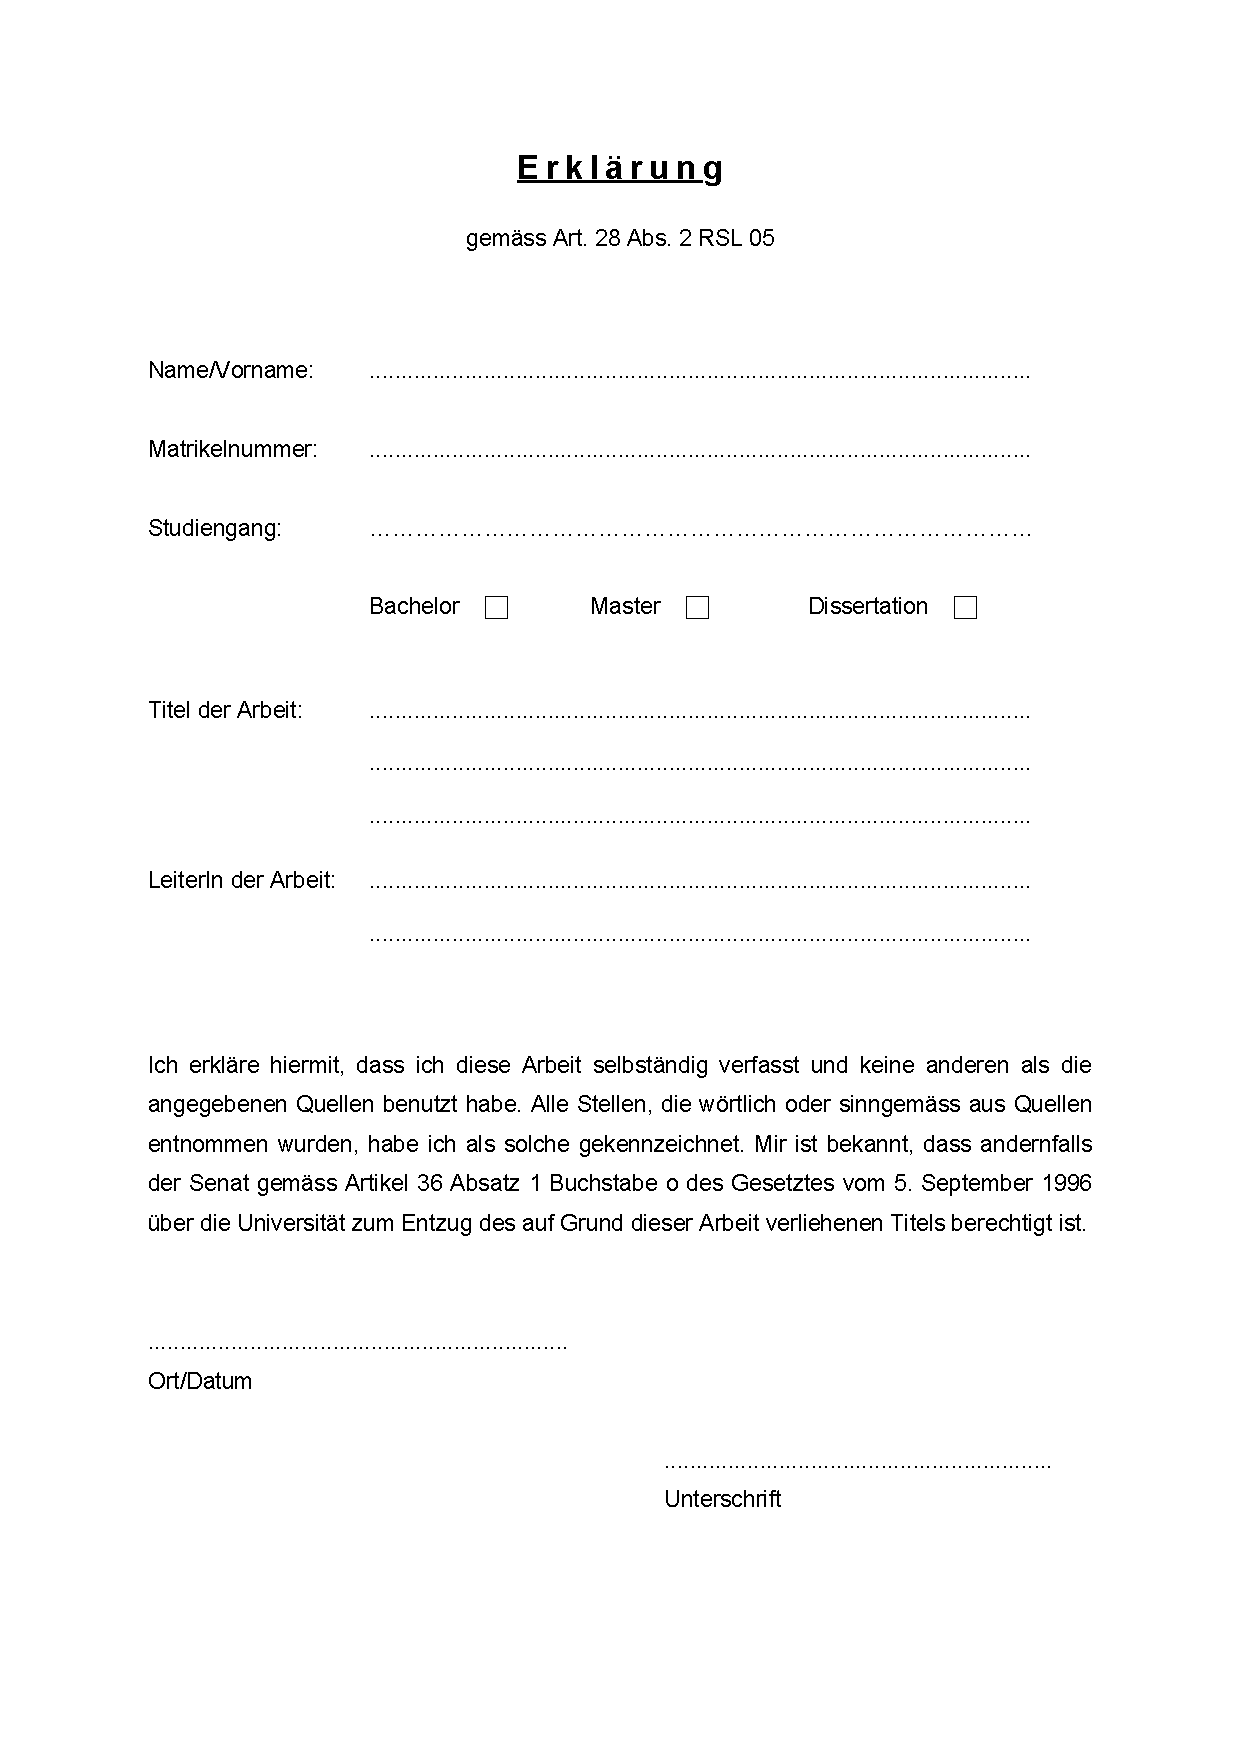
\includepdf{Erklaerung.pdf}


%END Doc
%-------------------------------------------------------

\end{document}
